% Options for packages loaded elsewhere
\PassOptionsToPackage{unicode}{hyperref}
\PassOptionsToPackage{hyphens}{url}
%
\documentclass[
  english,
  man]{apa6}
\title{\emph{Light Exposure Behavior Assessment (LEBA)}: Development of a novel instrument to capture light exposure-related behaviours}
\author{Mushfiqul Anwar Siraji\textsuperscript{1, *}, Rafael Robert Lazar\textsuperscript{2, 3, *}, Juliëtte van Duijnhoven\textsuperscript{4}, Luc Schlangen\textsuperscript{5}, Shamsul Haque\textsuperscript{1}, Vineetha Kalavally\textsuperscript{6}, Céline Vetter\textsuperscript{7, 8}, Gena Glickman\textsuperscript{9}, Karin Smolders\textsuperscript{10}, \& Manuel Spitschan\textsuperscript{11, 2, 3}}
\date{}

\usepackage{amsmath,amssymb}
\usepackage{lmodern}
\usepackage{iftex}
\ifPDFTeX
  \usepackage[T1]{fontenc}
  \usepackage[utf8]{inputenc}
  \usepackage{textcomp} % provide euro and other symbols
\else % if luatex or xetex
  \usepackage{unicode-math}
  \defaultfontfeatures{Scale=MatchLowercase}
  \defaultfontfeatures[\rmfamily]{Ligatures=TeX,Scale=1}
  \setmainfont[]{Arial}
\fi
% Use upquote if available, for straight quotes in verbatim environments
\IfFileExists{upquote.sty}{\usepackage{upquote}}{}
\IfFileExists{microtype.sty}{% use microtype if available
  \usepackage[]{microtype}
  \UseMicrotypeSet[protrusion]{basicmath} % disable protrusion for tt fonts
}{}
\makeatletter
\@ifundefined{KOMAClassName}{% if non-KOMA class
  \IfFileExists{parskip.sty}{%
    \usepackage{parskip}
  }{% else
    \setlength{\parindent}{0pt}
    \setlength{\parskip}{6pt plus 2pt minus 1pt}}
}{% if KOMA class
  \KOMAoptions{parskip=half}}
\makeatother
\usepackage{xcolor}
\IfFileExists{xurl.sty}{\usepackage{xurl}}{} % add URL line breaks if available
\IfFileExists{bookmark.sty}{\usepackage{bookmark}}{\usepackage{hyperref}}
\hypersetup{
  pdftitle={Light Exposure Behavior Assessment (LEBA): Development of a novel instrument to capture light exposure-related behaviours},
  pdfauthor={Mushfiqul Anwar Siraji1, *, Rafael Robert Lazar2, 3, *, Juliëtte van Duijnhoven4, Luc Schlangen5, Shamsul Haque1, Vineetha Kalavally6, Céline Vetter7, 8, Gena Glickman9, Karin Smolders10, \& Manuel Spitschan11, 2, 3},
  pdflang={en-EN},
  pdfkeywords={keywords},
  hidelinks,
  pdfcreator={LaTeX via pandoc}}
\urlstyle{same} % disable monospaced font for URLs
\usepackage{graphicx}
\makeatletter
\def\maxwidth{\ifdim\Gin@nat@width>\linewidth\linewidth\else\Gin@nat@width\fi}
\def\maxheight{\ifdim\Gin@nat@height>\textheight\textheight\else\Gin@nat@height\fi}
\makeatother
% Scale images if necessary, so that they will not overflow the page
% margins by default, and it is still possible to overwrite the defaults
% using explicit options in \includegraphics[width, height, ...]{}
\setkeys{Gin}{width=\maxwidth,height=\maxheight,keepaspectratio}
% Set default figure placement to htbp
\makeatletter
\def\fps@figure{htbp}
\makeatother
\setlength{\emergencystretch}{3em} % prevent overfull lines
\providecommand{\tightlist}{%
  \setlength{\itemsep}{0pt}\setlength{\parskip}{0pt}}
\setcounter{secnumdepth}{-\maxdimen} % remove section numbering
% Make \paragraph and \subparagraph free-standing
\ifx\paragraph\undefined\else
  \let\oldparagraph\paragraph
  \renewcommand{\paragraph}[1]{\oldparagraph{#1}\mbox{}}
\fi
\ifx\subparagraph\undefined\else
  \let\oldsubparagraph\subparagraph
  \renewcommand{\subparagraph}[1]{\oldsubparagraph{#1}\mbox{}}
\fi
\newlength{\cslhangindent}
\setlength{\cslhangindent}{1.5em}
\newlength{\csllabelwidth}
\setlength{\csllabelwidth}{3em}
\newlength{\cslentryspacingunit} % times entry-spacing
\setlength{\cslentryspacingunit}{\parskip}
\newenvironment{CSLReferences}[2] % #1 hanging-ident, #2 entry spacing
 {% don't indent paragraphs
  \setlength{\parindent}{0pt}
  % turn on hanging indent if param 1 is 1
  \ifodd #1
  \let\oldpar\par
  \def\par{\hangindent=\cslhangindent\oldpar}
  \fi
  % set entry spacing
  \setlength{\parskip}{#2\cslentryspacingunit}
 }%
 {}
\usepackage{calc}
\newcommand{\CSLBlock}[1]{#1\hfill\break}
\newcommand{\CSLLeftMargin}[1]{\parbox[t]{\csllabelwidth}{#1}}
\newcommand{\CSLRightInline}[1]{\parbox[t]{\linewidth - \csllabelwidth}{#1}\break}
\newcommand{\CSLIndent}[1]{\hspace{\cslhangindent}#1}
\usepackage{pdflscape}
\newcommand{\blandscape}{\begin{landscape}}
\newcommand{\elandscape}{\end{landscape}}
% Manuscript styling
\usepackage{upgreek}
\captionsetup{font=singlespacing,justification=justified}

% Table formatting
\usepackage{longtable}
\usepackage{lscape}
% \usepackage[counterclockwise]{rotating}   % Landscape page setup for large tables
\usepackage{multirow}		% Table styling
\usepackage{tabularx}		% Control Column width
\usepackage[flushleft]{threeparttable}	% Allows for three part tables with a specified notes section
\usepackage{threeparttablex}            % Lets threeparttable work with longtable

% Create new environments so endfloat can handle them
% \newenvironment{ltable}
%   {\begin{landscape}\centering\begin{threeparttable}}
%   {\end{threeparttable}\end{landscape}}
\newenvironment{lltable}{\begin{landscape}\centering\begin{ThreePartTable}}{\end{ThreePartTable}\end{landscape}}

% Enables adjusting longtable caption width to table width
% Solution found at http://golatex.de/longtable-mit-caption-so-breit-wie-die-tabelle-t15767.html
\makeatletter
\newcommand\LastLTentrywidth{1em}
\newlength\longtablewidth
\setlength{\longtablewidth}{1in}
\newcommand{\getlongtablewidth}{\begingroup \ifcsname LT@\roman{LT@tables}\endcsname \global\longtablewidth=0pt \renewcommand{\LT@entry}[2]{\global\advance\longtablewidth by ##2\relax\gdef\LastLTentrywidth{##2}}\@nameuse{LT@\roman{LT@tables}} \fi \endgroup}

% \setlength{\parindent}{0.5in}
% \setlength{\parskip}{0pt plus 0pt minus 0pt}

% \usepackage{etoolbox}
\makeatletter
\patchcmd{\HyOrg@maketitle}
  {\section{\normalfont\normalsize\abstractname}}
  {\section*{\normalfont\normalsize\abstractname}}
  {}{\typeout{Failed to patch abstract.}}
\patchcmd{\HyOrg@maketitle}
  {\section{\protect\normalfont{\@title}}}
  {\section*{\protect\normalfont{\@title}}}
  {}{\typeout{Failed to patch title.}}
\makeatother
\shorttitle{LEBA}
\keywords{keywords\newline\indent Word count: X}
\DeclareDelayedFloatFlavor{ThreePartTable}{table}
\DeclareDelayedFloatFlavor{lltable}{table}
\DeclareDelayedFloatFlavor*{longtable}{table}
\makeatletter
\renewcommand{\efloat@iwrite}[1]{\immediate\expandafter\protected@write\csname efloat@post#1\endcsname{}}
\makeatother
\usepackage{lineno}

\linenumbers
\usepackage{csquotes}
\ifXeTeX
  % Load polyglossia as late as possible: uses bidi with RTL langages (e.g. Hebrew, Arabic)
  \usepackage{polyglossia}
  \setmainlanguage[]{english}
\else
  \usepackage[main=english]{babel}
% get rid of language-specific shorthands (see #6817):
\let\LanguageShortHands\languageshorthands
\def\languageshorthands#1{}
\fi
\ifLuaTeX
  \usepackage{selnolig}  % disable illegal ligatures
\fi


\authornote{

Add complete departmental affiliations for each author here. Each new line herein must be indented, like this line.

Enter author note here.

The authors made the following contributions. Mushfiqul Anwar Siraji: Formal Analysis, Visualization, Writing -- original draft, Writing -- review \& editing;; Rafael Robert Lazar: Data curation, Investigation, Project administration, Visualization, Writing -- original draft, Writing -- review \& editing;; Juliëtte van Duijnhoven: Conceptualization, Methodology, Investigation, Writing -- review \& editing; Luc Schlangen: Conceptualization, Methodology, Investigation, Writing -- review \& editing; Shamsul Haque: Conceptualization, Supervision, Writing -- review \& editing; Vineetha Kalavally: Supervision, Writing -- review \& editing; Céline Vetter: Conceptualization, Writing -- review \& editing; Gena Glickman: Conceptualization, Methodology, Writing -- review \& editing; Karin Smolders: Conceptualization, Methodology, Writing -- review \& editing; Manuel Spitschan: Conceptualization, Data curation, Investigation, Project administration, Visualization, Methodology, Writing -- original draft, Writing -- review \& editing.

}

\affiliation{\vspace{0.5cm}\textsuperscript{1} Monash University, Department of Psychology, Jeffrey Cheah School of Medicine and Health Sciences, Malaysia\\\textsuperscript{2} Psychiatric Hospital of the University of Basel (UPK), Centre for Chronobiology, Basel, Switzerland\\\textsuperscript{3} University of Basel, Transfaculty Research Platform Molecular and Cognitive Neurosciences, Basel, Switzerland\\\textsuperscript{4} Eindhoven University of Technology, Department of the Built Environment, Building Lighting, Eindhoven, Netherlands\\\textsuperscript{5} Eindhoven University of Technology, Department of Industrial Engineering and Innovation Sciences, Intelligent Lighting Institute, Eindhoven, Netherlands\\\textsuperscript{6} Monash University, Department of Electrical and Computer Systems Engineering, Malaysia, Selangor, Malaysia\\\textsuperscript{7} University of Colorado Boulder, Department of Integrative Physiology, Boulder, USA\\\textsuperscript{8} Ximes GmbH, Frankfurt, Germany\\\textsuperscript{9} Uniformed Services University of the Health Sciences, Department of Psychiatry, Bethesda, USA\\\textsuperscript{10} Eindhoven University of Technology, Human-Technology Interaction Group, Eindhoven, Netherlands\\\textsuperscript{11} University of Oxford, Department of Experimental Psychology, Oxford, UK\\\textsuperscript{*} Joint first author}

\abstract{
One or two sentences providing a \textbf{basic introduction} to the field, comprehensible to a scientist in any discipline.

Two to three sentences of \textbf{more detailed background}, comprehensible to scientists in related disciplines.

One sentence clearly stating the \textbf{general problem} being addressed by this particular study.

One sentence summarizing the main result (with the words ``\textbf{here we show}'' or their equivalent).

Two or three sentences explaining what the \textbf{main result} reveals in direct comparison to what was thought to be the case previously, or how the main result adds to previous knowledge.

One or two sentences to put the results into a more \textbf{general context}.

Two or three sentences to provide a \textbf{broader perspective}, readily comprehensible to a scientist in any discipline.
}



\begin{document}
\maketitle

\hypertarget{introduction}{%
\section{Introduction}\label{introduction}}

\begin{itemize}
\item
  Light exposure is important
\item
  Light exposure Behavior is important
\item
  Table: Overview Existing Related Scales: items in total / items on light exposure (behaviour)
\item
  Existing Scales: Review them in text
\item
  None of these do light exposure behavior.
\end{itemize}

\begin{longtable}[t]{>{\raggedright\arraybackslash}p{4cm}>{\raggedright\arraybackslash}p{4cm}>{\raggedright\arraybackslash}p{4cm}>{\raggedright\arraybackslash}p{4cm}}
\caption{\label{tab:unnamed-chunk-2}Releated Scales}\\
\toprule
Name & Author & Description & Relevant Items\\
\midrule
\endfirsthead
\caption[]{\label{tab:unnamed-chunk-2}Releated Scales \textit{(continued)}}\\
\toprule
Name & Author & Description & Relevant Items\\
\midrule
\endhead

\endfoot
\bottomrule
\endlastfoot
Visual Light Sensitivity Questionnaire-8 & Verriotto et al., 2017 & Eight-question survey to assess the presence and severity of photosensitivity symptoms & NA\\
Office Light Survey & Eklundet al., 1996 & A survey to assess electrical lighting environment in office & NA\\
Harvard Light Exposure Assessment Questionnaire & Bajaj et al., 2011 & Self-administered semi-quantitative light questionnaire & NA\\
Hospital Lighting Survey & Dianat et el.,.2013 & 23 items questionnaire to assess light environment in a hospital & NA\\
Morningness-Eveningness Questionnaire & Horne et al.,1976 & 19 items questionnaire to understand your body clock & NA\\
\addlinespace
Munich Chronotype Questionnaire (MCTQ) & Roenneberg et al.,2003 & 17 items questionnaire to understand individuals phase of entrainment & NA\\
Assessment of Sleep Environment & Olivier et.al.,.2016] & 13 items questionnaire measuring your sleep environment quality & NA\\
The Pittsburgh Sleep Quality Index (PSQI) & Buysse ei al.,1989 & 9 items inventory to measure sleep quality and sleeping pattern & NA\\
Self-Rating of Biological Rhythm Disorder for Adolescents (SBRDA) & Xie et al.,2021 & 29 Items questionnaire assessing four dimensions of biological rhythm disorder in adolescents & Item 3,22-25 and 29\\
Photosensitivity Assessment Questionnaire (PAQ) & Wu et al.,2017 & 16 dichotomous (yes/no) items questionnaire to assess "photophobia" and "photophilia" & All itms\\*
\end{longtable}

\hypertarget{methods}{%
\section{Methods}\label{methods}}

\hypertarget{ethical-approval}{%
\subsection{Ethical approval}\label{ethical-approval}}

The cantonal ethics commission (Ethikkommission Nordwest- und Zentralschweiz, project ID Req-2021-00488) reviewed this project and issued an official clarification of responsibility (full document see Suppl. Fig X in appendix) stating: ``The research project does not fall under the scope of the Human Research Act, because your project is using only anonymised data. An authorisation from the ethics committee is therefore not required and the EKNZ is not responsible for its review.''

\hypertarget{data-availability}{%
\subsection{Data Availability}\label{data-availability}}

\hypertarget{survey-characteristics}{%
\subsection{Survey characteristics}\label{survey-characteristics}}

Data was collected in a quantitative cross-sectional approach via a fully anonymous online survey hosted on REDCap (Harris et al., 2019, 2009) by way of the University of Basel \href{https://redcap.scicore.unibas.ch}{sciCORE}. Participants were recruited via the \href{https://enlightenyourclock.org/participate-in-research}{website} of a Comic co-released with the survey(Weinzaepflen \& Spitschan, 2021) , social media (i.e., LinkedIn, Twitter, Facebook), mailing lists, word of mouth, the investigators' personal contacts, and supported by distribution of the survey link via f.lux software (F.lux Software LLC, 2021).

Completing the online survey took approx. 15 to 20 minutes and was not compensated. The first page of the survey comprised a participant information sheet, where participants' informed consent to participate was obtained before any of the questions were displayed. Underaged participants (\textless18 years) were urged to obtain assent from their parents/legal guardians, before filling in the survey. Information on the first page included the objectives of the study, inclusion criteria, estimated duration, the use, storage and sharing of the data, compensation (none), and information about the type of questions in the survey. Moreover, participants needed to confirm that they were participating the survey for the first time. To ensure high data quality, five attention check items were included in the survey (e.g., ``We want to make sure you are paying attention. What is 4+5?''). The data analysed in this study was collected between 17.05.2021 and 03.09.2021. Questions incorporating retrospective recall were all aligned to the period of ``past four weeks,'' matching the presented LEBA instrument.

In addition to the LEBA questionnaire, which is subject of the current study, the following variables and items were assessed but not included in the analysis:

\begin{itemize}
\tightlist
\item
  Sleep disturbance and sleep-related impairment (adult and pediatric versions) (Bevans et al., 2019; Daniel J. Buysse et al., 2010; Forrest et al., 2018; Harb, Hidalgo, \& Martau, 2015; L. Yu et al., 2011)
\item
  Sleep duration, timing, and latency, chronotype, social jetlag, time in bed, work/sleep schedule and outdoor light exposure duration (version for adults and adolescents) (Roenneberg, Wirz-Justice, \& Merrow, 2003)
\item
  Sleep environment (Olivier et al., 2016)
\item
  Meal timing \& caffeine consumption {[}custom items{]}
\item
  Light sensitivity (photophobia vs.~photophilia) (Wu \& Hallett, 2017)
\item
  Self-reported pubertal stage (only if younger than 18 years old) (Petersen, Crockett, Richards, \& Boxer, 1988)
\end{itemize}

Furthermore, the following 1-item demographic variables were assessed:

\begin{itemize}
\tightlist
\item
  Age
\item
  Sex
\item
  Gender identity
\item
  Occupational Status
\item
  COVID-19 related Occupational setting during the past four weeks
\item
  Time zone \& country of residence
\item
  English as native language
\end{itemize}

\hypertarget{participants}{%
\subsection{Participants}\label{participants}}

\begin{table}

\caption{\label{tab:prepareDescTable}Dempgraphics}
\centering
\resizebox{\linewidth}{!}{
\begin{tabular}[t]{llllll}
\toprule
Variable & Overall, N = 690 & 1. EFA Sample, N = 428 & 2. CFA Sample, N = 262 & p-value & q-value\\
\midrule
Age & 32.95 (14.57) & 32.99 (15.11) & 32.89 (13.66) & 0.5 & 0.5\\
Sex &  &  &  & 0.14 & 0.4\\
\hspace{1em}Female & 325 (47\%) & 189 (44\%) & 136 (52\%) &  & \\
\hspace{1em}Male & 351 (51\%) & 230 (54\%) & 121 (46\%) &  & \\
\hspace{1em}Other & 14 (2.0\%) & 9 (2.1\%) & 5 (1.9\%) &  & \\
\addlinespace
Gender-Variant Identity & 49 (7.2\%) & 33 (7.8\%) & 16 (6.2\%) & 0.4 & 0.5\\
Native English Speaker & 320 (46\%) & 191 (45\%) & 129 (49\%) & 0.2 & 0.5\\
Occupational Status &  &  &  & 0.040 & 0.2\\
\hspace{1em}Work & 396 (57\%) & 235 (55\%) & 161 (61\%) &  & \\
\hspace{1em}School & 174 (25\%) & 122 (29\%) & 52 (20\%) &  & \\
\addlinespace
\hspace{1em}Neither & 120 (17\%) & 71 (17\%) & 49 (19\%) &  & \\
Occupational setting &  &  &  & 0.3 & 0.5\\
\hspace{1em}Home office/Home schooling & 303 (44\%) & 194 (45\%) & 109 (42\%) &  & \\
\hspace{1em}Face-to-face work/Face-to-face schooling & 109 (16\%) & 68 (16\%) & 41 (16\%) &  & \\
\hspace{1em}Combination of home- and face-to-face- work/schooling & 147 (21\%) & 94 (22\%) & 53 (20\%) &  & \\
\addlinespace
\hspace{1em}Neither (no work or school, or in vacation) & 131 (19\%) & 72 (17\%) & 59 (23\%) &  & \\
\bottomrule
\multicolumn{6}{l}{\rule{0pt}{1em}\textsuperscript{1} Mean (SD); n (\%)}\\
\multicolumn{6}{l}{\rule{0pt}{1em}\textsuperscript{2} Wilcoxon rank sum test; Pearson's Chi-squared test}\\
\multicolumn{6}{l}{\rule{0pt}{1em}\textsuperscript{3} False discovery rate correction for multiple testing}\\
\end{tabular}}
\end{table}

Table 1 summarizes the survey participants' demographic characteristics. Only participants completing the full LEBA questionnaire were included, thus there are no missing values in the item analyses. XX participants were excluded from analysis due to not passing at least one of the ``attention check'' items. For exploring initial factor structure (EFA) , a sample of 250-300 is recommended (Comrey \& Lee, 1992; Schönbrodt \& Perugini, 2013). For estimating the sample size for the confirmatory factor analysis (CFA) we followed the N:q rule (Bentler \& Chou, 1987; Jackson, 2003; Kline, 2015; Worthington \& Whittaker, 2006), where ten participants per parameter is required to earn trustworthiness of the result. Our sample size exceeds these requirements: Anonymous responses from a total of \emph{n} = 690 participants were included in the analysis of the current study, split into samples for exploratory (EFA: \emph{n} = 428) and confirmatory factor analysis (CFA: \emph{n} = 262). The EFA sample included participants filling out the questionnaire from 17.05.2021 to XX.XX.XXXX , whereas participants who filled out the questionnaire from YY.YY.YYYY to 03.09.2021 were included in the CFA analysis. Participants indicated filling out the online survey from a diverse range of geographic locations. The four most common geographic locations included:

\begin{tabular}{l|r}
\hline
  & x\\
\hline
United States - America/New\_York (UTC -04:00) & 63\\
\hline
United Kingdom - Europe/London (UTC) & 57\\
\hline
Germany - Europe/Berlin (UTC +01:00) & 53\\
\hline
India - Asia/Kolkata (UTC +05:30) & 38\\
\hline
\end{tabular}

For a full list of geographic locations, see Suppl. Table X in the appendix.

Age among all participants ranged from 11 years to 84 years {[}EFA: \emph{min} = 11, \emph{max} = 84; CFA: \emph{min} = 12, \emph{max} = 74{]}, with an overall mean of \textasciitilde{} 33 years of age {[}Overall: \emph{M} = 32.95, \emph{SD} = 14.57; EFA: \emph{M} = 32.99, \emph{SD} = 15.11; CFA: \emph{M} = 32.89, \emph{SD} = 13.66{]}. In total 325 (47\%) of the participants indicated female sex {[}EFA: 189 (44\%); CFA: 136 (52\%){]}, 351 (51\%) indicated male {[}EFA: 230 (54\%); CFA: 121 (46\%){]} and 14 (2.0\%) indicated other sex {[}EFA: 9 (2.1\%), CFA: 5 (1.9\%){]}. Overall, 49 (7.2\%) {[}EFA: 33 (7.8\%); CFA: 16 (6.2\%){]} participants indicated a gender-variant identity. In a ``Yes/No'' question regarding native language, 320 (46\%) of respondents {[}EFA: 191 (45\%); CFA: 129 (49\%){]} indicated to be native English speakers. For their ``Occupational Status,'' more than half of the overall sample reported that they currently work {[}Overall: 396 (57\%); EFA: 235 (55\%); CFA: 161 (61\%){]}, whereas 174 (25\%) {[}EFA: 122 (29\%); CFA: 52 (20\%){]} reported that they go to school and 120 (17\%) {[}EFA: 71 (17\%); CFA: 49 (19\%){]} responded that they do ``Neither.'' With respect to the COVID-19 pandemic we asked participants to indicate their occupational setting during the last four weeks: In the overall sample 303 (44\%) {[}EFA: 194 (45\%); CFA: 109 (42\%){]} of the participants indicated that they were in a home office/ home schooling setting., while 109 (16\%) overall {[}EFA: 68 (16\%) ; CFA: 41 (16\%){]} reported face-to-face work/schooling. Lastly, 147 (21\%) overall {[}EFA: 94 (22\%) ; CFA: 53 (20\%){]} reported a combination of home- and face-to-face work/schooling, whereas 131 (19\%) overall {[}EFA: 72 (17\%); CFA: 59 (23\%){]} filled in the ``Neither (no work or school, or indication)'' response option. We tested all demographic variables in Table 1 for significant group differences between the EFA and CFA sample, applying Wilcoxon rank sum test for the continuous variable ``Age'' and Pearson's \(\chi^2\) test for all other categorical variables via the gtsummary R package's ``add\_p'' function (Sjoberg et al., 2021a) . The p-values were corrected for multiple testing applying false discovery rate (FDR) via the ``add\_q'' function of the same package. After p-value (FDR) correction for multiple testing, none of the demographic variables were significantly different between the EFA sample and the CFA sample (all q-values \emph{q} ≥ 0.2 , indicating equivalence).

\begin{enumerate}
\def\labelenumi{\arabic{enumi}.}
\tightlist
\item
  Describe EFA and CFA sample separately.
\item
  Sampling technique: Convince sampling (non-probability sample)
\item
  Method: cross-sectional survey
\item
  How many missing data?
\item
  How incomplete data were addressed.
\item
  Why such sample was chosen?
\end{enumerate}

\hypertarget{procedure}{%
\subsection{Procedure}\label{procedure}}

\hypertarget{development-of-the-scale}{%
\subsubsection{Development of the Scale}\label{development-of-the-scale}}

\begin{enumerate}
\def\labelenumi{\arabic{enumi}.}
\tightlist
\item
  How the items were generated
\item
  How the literature was reviewed to identify construct adequacy of the items.
\item
  Discuss the expert panel review process to assess content validity
\end{enumerate}

\begin{figure}

{\centering 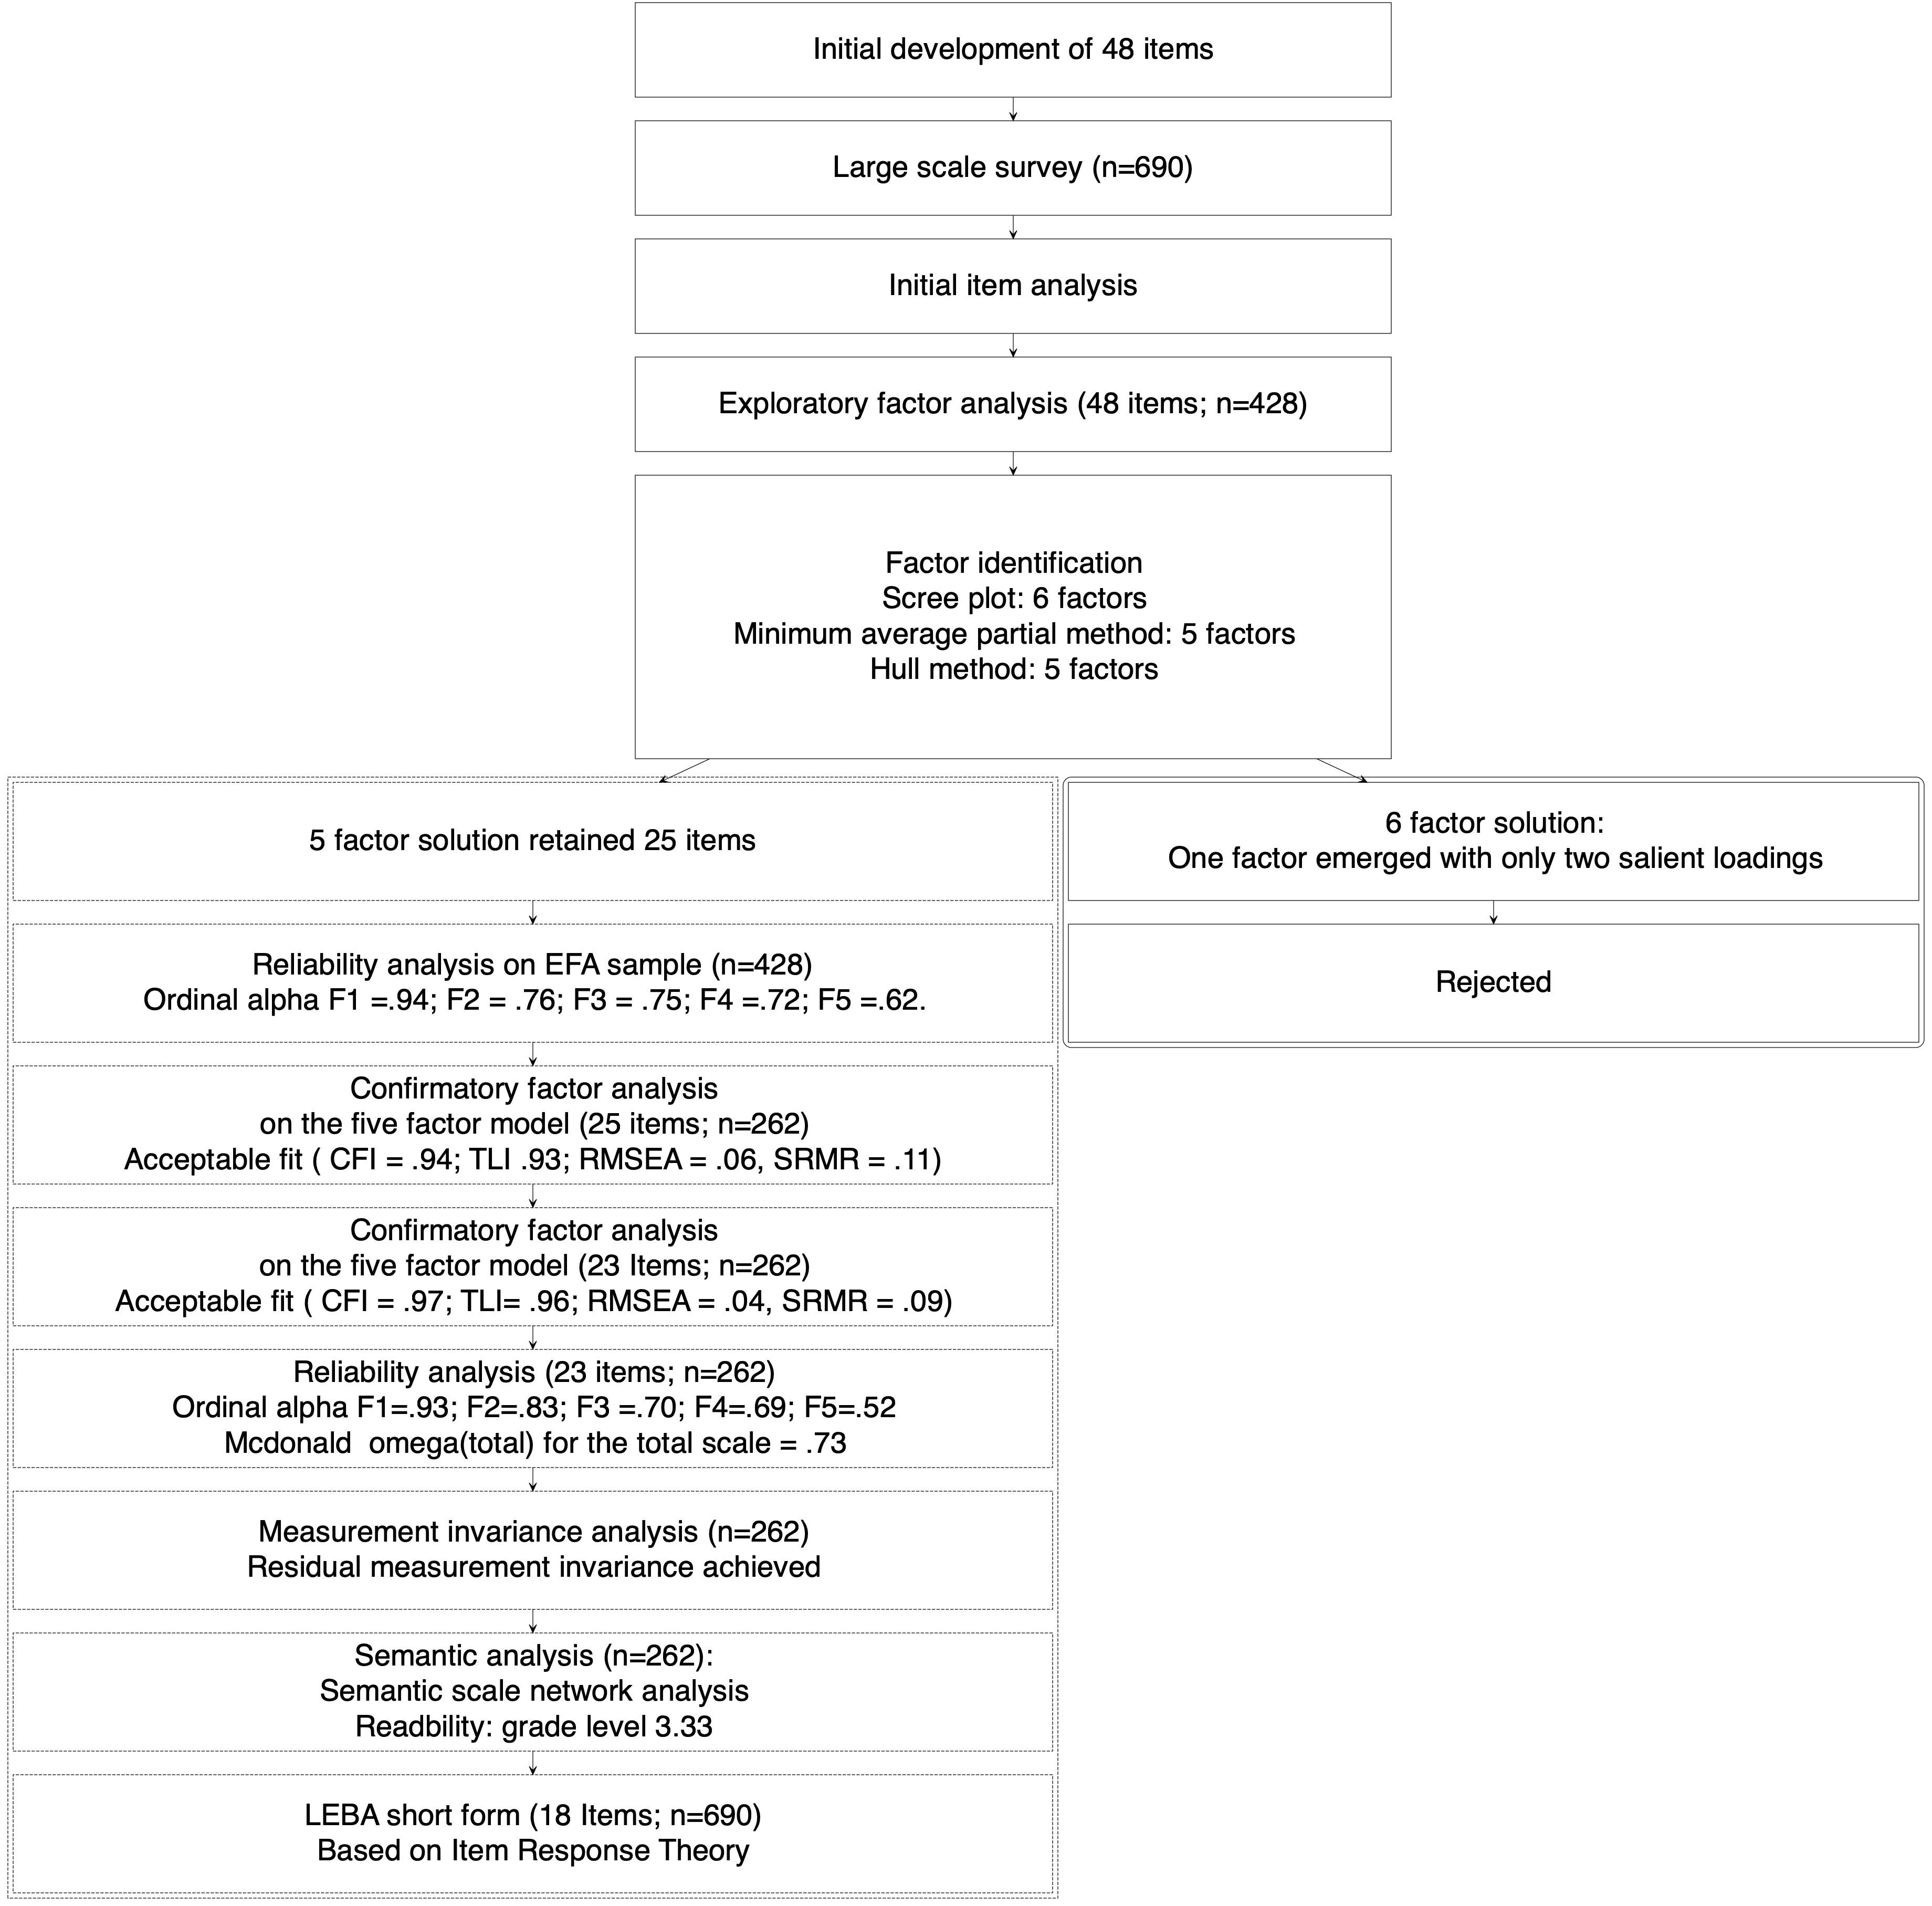
\includegraphics[width=1\linewidth,height=1\textheight]{Manuscript.figures/Flowchart1} 

}

\caption{Development of LEBA}\label{fig:FlowchartFig}
\end{figure}

\hypertarget{data-collection}{%
\subsubsection{Data Collection}\label{data-collection}}

Timeline of data collection, mode of data collection.

\hypertarget{analytic-strategies}{%
\subsection{Analytic Strategies}\label{analytic-strategies}}

We used R (version 4.1.0), including several R packages, for our analyses.Initially, our tool have six point Likert type response scale (0:Does not apply/I don't know; 1:Never, 2:Rarely; 3:Sometimes; 4:Often; 5: Always). As our purpose was to capture light exposure related behavior, ``Does not apply/I don't know'' and ``Never'' were providing similar information. As such we decided to collapse ``Does not apply/I don't know'' and ``Never'' options into one making it a 5 point Likert type response scale. Necessary assumptions of EFA, including sample adequacy, normality assumptions, quality of correlation matrix, were assessed. Our data violated both the univariate and multivariate normality assumptions. Due to these violations and the ordinal nature of our response data, we used a polychoric correlation matrix (C. Desjardins \& Bulut, 2018) for the EFA. We employed principal axis (PA) as a factor extraction method with varimax rotation. PA is robust to the normality assumption violations (Watkins, 2020). The obtained latent structure was confirmed by another factor extraction method: the minimum residuals extraction method as well. We used a combination factor identification method including scree plot(Cattell, 1966), Horn's parallel analysis (Horn, 1965), minimum average partials method(Velicer, 1976), and hull method (Lorenzo-Seva, Timmerman, \& Kiers, 2011) to identify factor numbers. Additionally, to determine the simple structure, we followed the following guidelines recommended by psychometricians (i) no factors with fewer than three items (ii) no factors with a factor loading \textless0.3 (iii) no items with cross-loading greater than .3 across factors (Bandalos \& Finney, 2018) We also conducted psychometric analysis on non-merged response options data (supplementary analysis) and rejected the latent structure obtained as the factors were less interpretable.

\hypertarget{results}{%
\section{Results}\label{results}}

\hypertarget{exploratory-factor-analysis}{%
\subsection{Exploratory Factor Analysis}\label{exploratory-factor-analysis}}

Sampling adequacy was checked using Kaiser-Meyer-Olkin (KMO) measures of sampling adequacy(Kaiser, 1974) . The overall KMO vale for 48 items was 0.63 which was above the cutoff value (.50) indicating a mediocre sample (Hutcheson, 1999). Table\ref{tab:tabDes} summarizes the univariate descriptive statistics for the 48 items. some of the items were skewed with high Kurtosis values. Our data violated both univariate normality (Shapiro-Wilk statistics; (Shapiro \& Wilk, 1965)) and multivariate normality assumptions (Marida's test;(Mardia, 1970)). Multivariate skew was = 583.80 (p \textless0.001) and multivariate kurtosis was = 2,749.15 (p \textless0.001). Due to these violations and ordinal nature of the response data polychoric correlations over Pearson's correlations was chosen (C. Desjardins \& Bulut, 2018). Bartlett's test of sphericity (Bartlett, 1954), \(\chi^2\) (1128) = 5042.86, p \textless{} .001{]} indicated the correlations between items are adequate for the EFA. However only 4.96\% of the inter-item correlation coefficients were greater than .30. The inter item correlation ranged between .44 to .91. And the corrected item-total correlations ranged between .10 to .44.

\begin{center}
\begin{ThreePartTable}

\begin{TableNotes}[para]
\normalsize{\textit{Note.} *p<.001}
\end{TableNotes}

\begin{longtable}{ccccccc}\noalign{\getlongtablewidth\global\LTcapwidth=\longtablewidth}
\caption{\label{tab:tabDes}Descriptive Statistics}\\
\toprule
 & \multicolumn{1}{c}{Mean} & \multicolumn{1}{c}{SD} & \multicolumn{1}{c}{Skew} & \multicolumn{1}{c}{Kurtosis} & \multicolumn{1}{c}{Shapiro-Wilk Statistics} & \multicolumn{1}{c}{Item-Total Correlation}\\
\midrule
\endfirsthead
\caption*{\normalfont{Table \ref{tab:tabDes} continued}}\\
\toprule
 & \multicolumn{1}{c}{Mean} & \multicolumn{1}{c}{SD} & \multicolumn{1}{c}{Skew} & \multicolumn{1}{c}{Kurtosis} & \multicolumn{1}{c}{Shapiro-Wilk Statistics} & \multicolumn{1}{c}{Item-Total Correlation}\\
\midrule
\endhead
Item1 & 2.27 & 1.39 & 0.74 & -0.81 & 0.81* & .25\\
Item2 & 2.87 & 1.59 & 0.08 & -1.60 & 0.83* & .19\\
Item3 & 3.36 & 1.38 & -0.48 & -1.03 & 0.87* & .16\\
Item4 & 1.47 & 1.18 & 2.38 & 4.00 & 0.43* & .28\\
Item5 & 4.01 & 1.40 & -1.22 & 0.07 & 0.70* & .13\\
Item6 & 2.79 & 1.55 & 0.19 & -1.48 & 0.85* & .20\\
Item7 & 2.26 & 1.25 & 0.70 & -0.60 & 0.85* & .19\\
Item8 & 2.97 & 1.20 & -0.06 & -0.94 & 0.91* & -.10\\
Item9 & 2.94 & 1.03 & -0.12 & -0.40 & 0.91* & .10\\
Item10 & 2.74 & 1.04 & 0.09 & -0.74 & 0.91* & .28\\
Item11 & 2.18 & 0.90 & 0.60 & 0.12 & 0.86* & .26\\
Item12 & 2.36 & 1.22 & 0.59 & -0.62 & 0.87* & .25\\
Item13 & 2.73 & 1.46 & 0.20 & -1.36 & 0.87* & .33\\
Item14 & 2.14 & 1.31 & 0.77 & -0.78 & 0.80* & .26\\
Item15 & 3.26 & 1.09 & -0.26 & -0.45 & 0.91* & .14\\
Item16 & 1.56 & 1.23 & 2.00 & 2.45 & 0.50* & .32\\
Item17 & 1.54 & 1.21 & 2.07 & 2.75 & 0.49* & .31\\
Item18 & 1.12 & 0.49 & 5.02 & 27.80 & 0.25* & .16\\
Item19 & 1.05 & 0.36 & 7.23 & 52.98 & 0.13* & .18\\
Item20 & 1.04 & 0.33 & 8.99 & 85.28 & 0.10* & .16\\
Item21 & 1.14 & 0.59 & 4.79 & 24.05 & 0.25* & .16\\
Item22 & 3.57 & 1.07 & -0.65 & -0.17 & 0.88* & .21\\
Item23 & 2.56 & 1.27 & 0.33 & -1.00 & 0.89* & .11\\
Item24 & 4.14 & 0.99 & -1.23 & 1.14 & 0.79* & .19\\
Item25 & 2.59 & 1.41 & 0.27 & -1.27 & 0.86* & .19\\
Item26 & 2.25 & 1.27 & 0.69 & -0.64 & 0.84* & .18\\
Item27 & 3.80 & 1.29 & -0.87 & -0.42 & 0.82* & .17\\
Item28 & 3.76 & 1.14 & -0.68 & -0.45 & 0.86* & .00\\
Item29 & 2.44 & 1.31 & 0.38 & -1.14 & 0.86* & .11\\
Item30 & 1.48 & 1.11 & 2.18 & 3.35 & 0.48* & .24\\
Item31 & 3.00 & 1.62 & -0.08 & -1.61 & 0.83* & .44\\
Item32 & 3.55 & 1.65 & -0.60 & -1.34 & 0.76* & .43\\
Item33 & 3.62 & 1.64 & -0.68 & -1.25 & 0.74* & .32\\
Item34 & 3.42 & 1.83 & -0.45 & -1.69 & 0.69* & .33\\
Item35 & 3.86 & 1.67 & -0.99 & -0.85 & 0.65* & .23\\
Item36 & 1.54 & 1.25 & 2.13 & 2.86 & 0.46* & .36\\
Item37 & 1.33 & 0.91 & 3.03 & 8.43 & 0.41* & .01\\
Item38 & 4.30 & 1.08 & -1.79 & 2.53 & 0.67* & .22\\
Item39 & 1.96 & 0.98 & 1.02 & 0.69 & 0.82* & .05\\
Item40 & 2.16 & 1.19 & 0.71 & -0.54 & 0.84* & .14\\
Item41 & 1.31 & 0.81 & 2.75 & 6.92 & 0.43* & .21\\
Item42 & 3.93 & 1.48 & -1.06 & -0.44 & 0.71* & .18\\
Item43 & 1.64 & 1.18 & 1.79 & 2.02 & 0.60* & .15\\
Item44 & 3.51 & 1.30 & -0.70 & -0.59 & 0.85* & .39\\
Item45 & 2.22 & 1.48 & 0.71 & -1.02 & 0.76* & .30\\
Item46 & 1.76 & 1.23 & 1.35 & 0.44 & 0.66* & .38\\
Item47 & 2.11 & 1.17 & 0.77 & -0.39 & 0.83* & .32\\
Item48 & 2.60 & 1.25 & 0.29 & -0.86 & 0.89* & .35\\
\bottomrule
\addlinespace
\insertTableNotes
\end{longtable}

\end{ThreePartTable}
\end{center}

\begin{figure}

{\centering 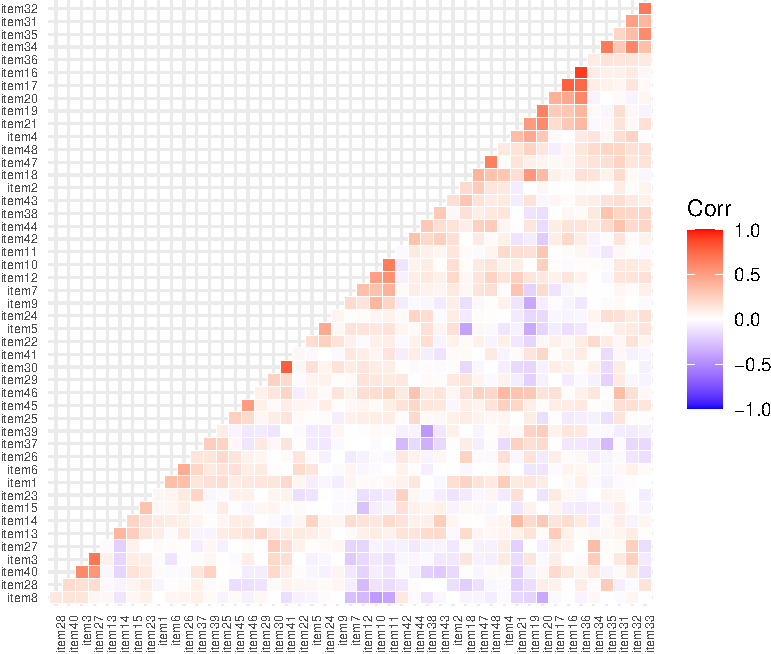
\includegraphics[width=1\linewidth]{manuscript_files/figure-latex/figCor-1} 

}

\caption{Correlation plot of the items}\label{fig:figCor}
\end{figure}

Scree plot ( Figure \ref{fig:facIdFig}) suggested a six-factor solution. Horn's parallel analysis (Horn, 1965) with 500 iterations also indicated a six-factor solution. However, the minimum average partial (MAP) method (Velicer, 1976) and Hull method (Lorenzo-Seva et al., 2011) suggested a five-factor solution. As a result, we tested both five-factor and six-factor solutions.

\begin{figure}

{\centering 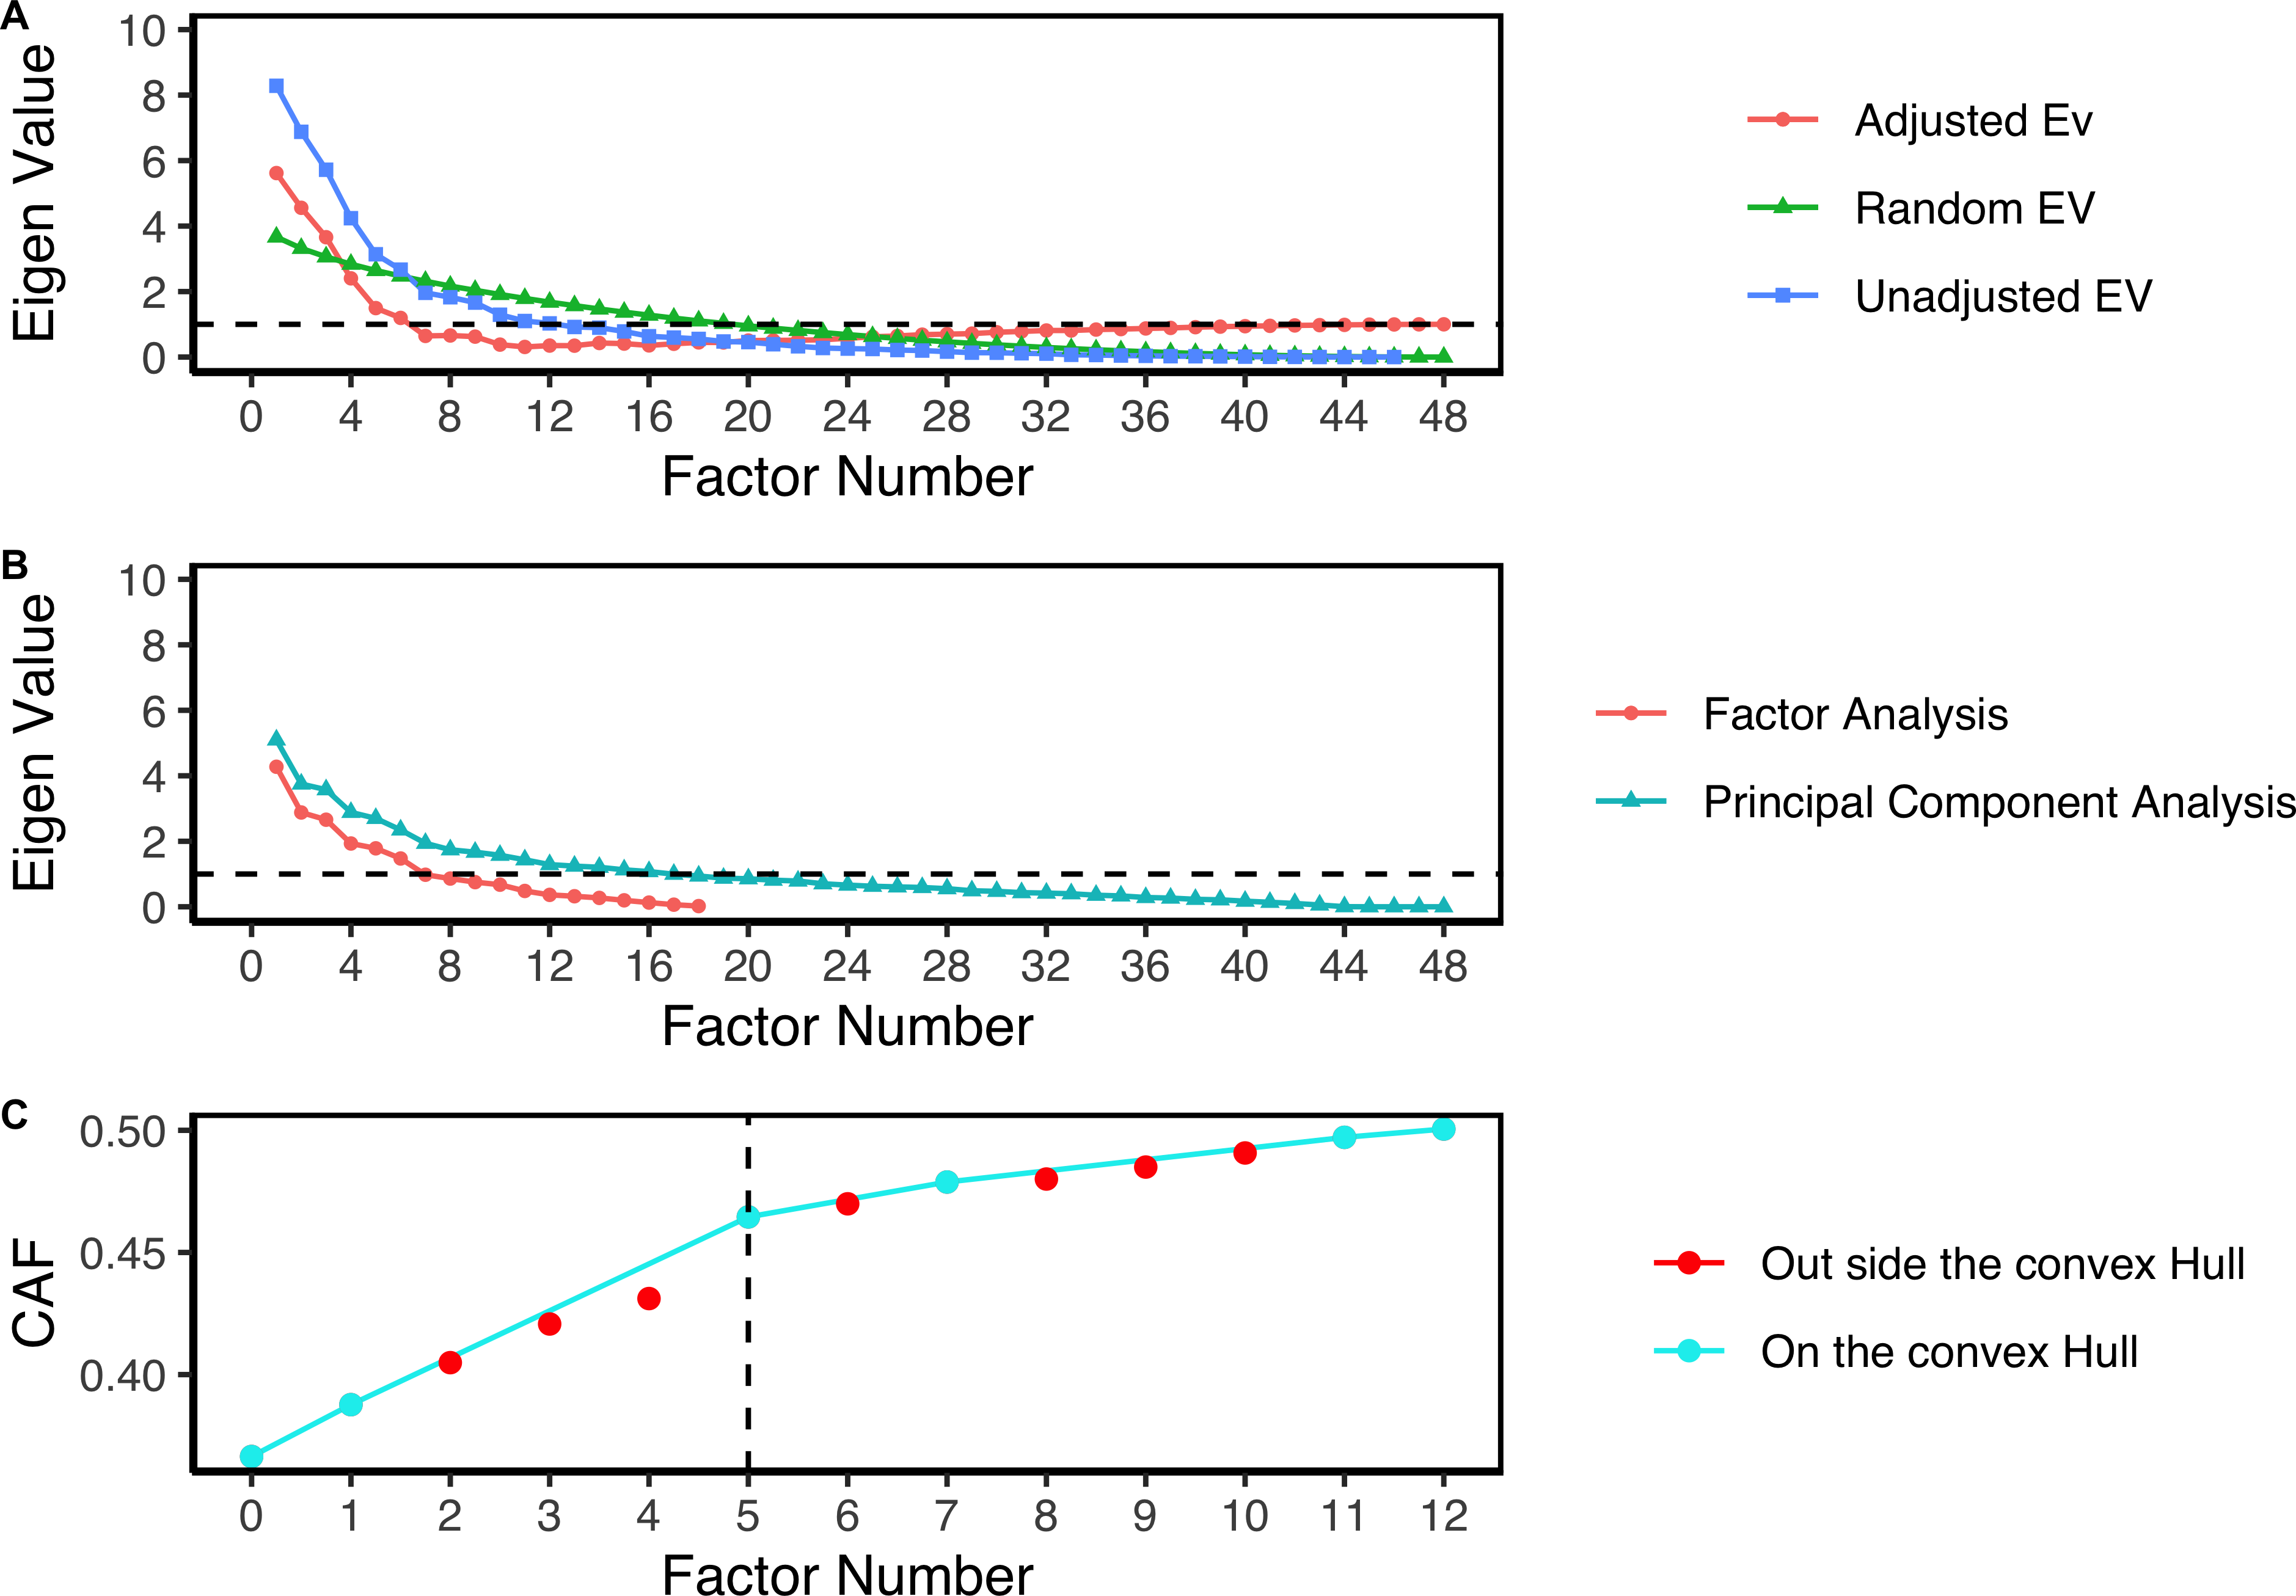
\includegraphics[width=1\linewidth,height=2\textheight]{manuscript_files/figure-latex/facIdFig-1} 

}

\caption{Factor Identification (A) Parallel analysis (B) Scree Plot (C) Hull Method}\label{fig:facIdFig}
\end{figure}

\begin{figure}

{\centering 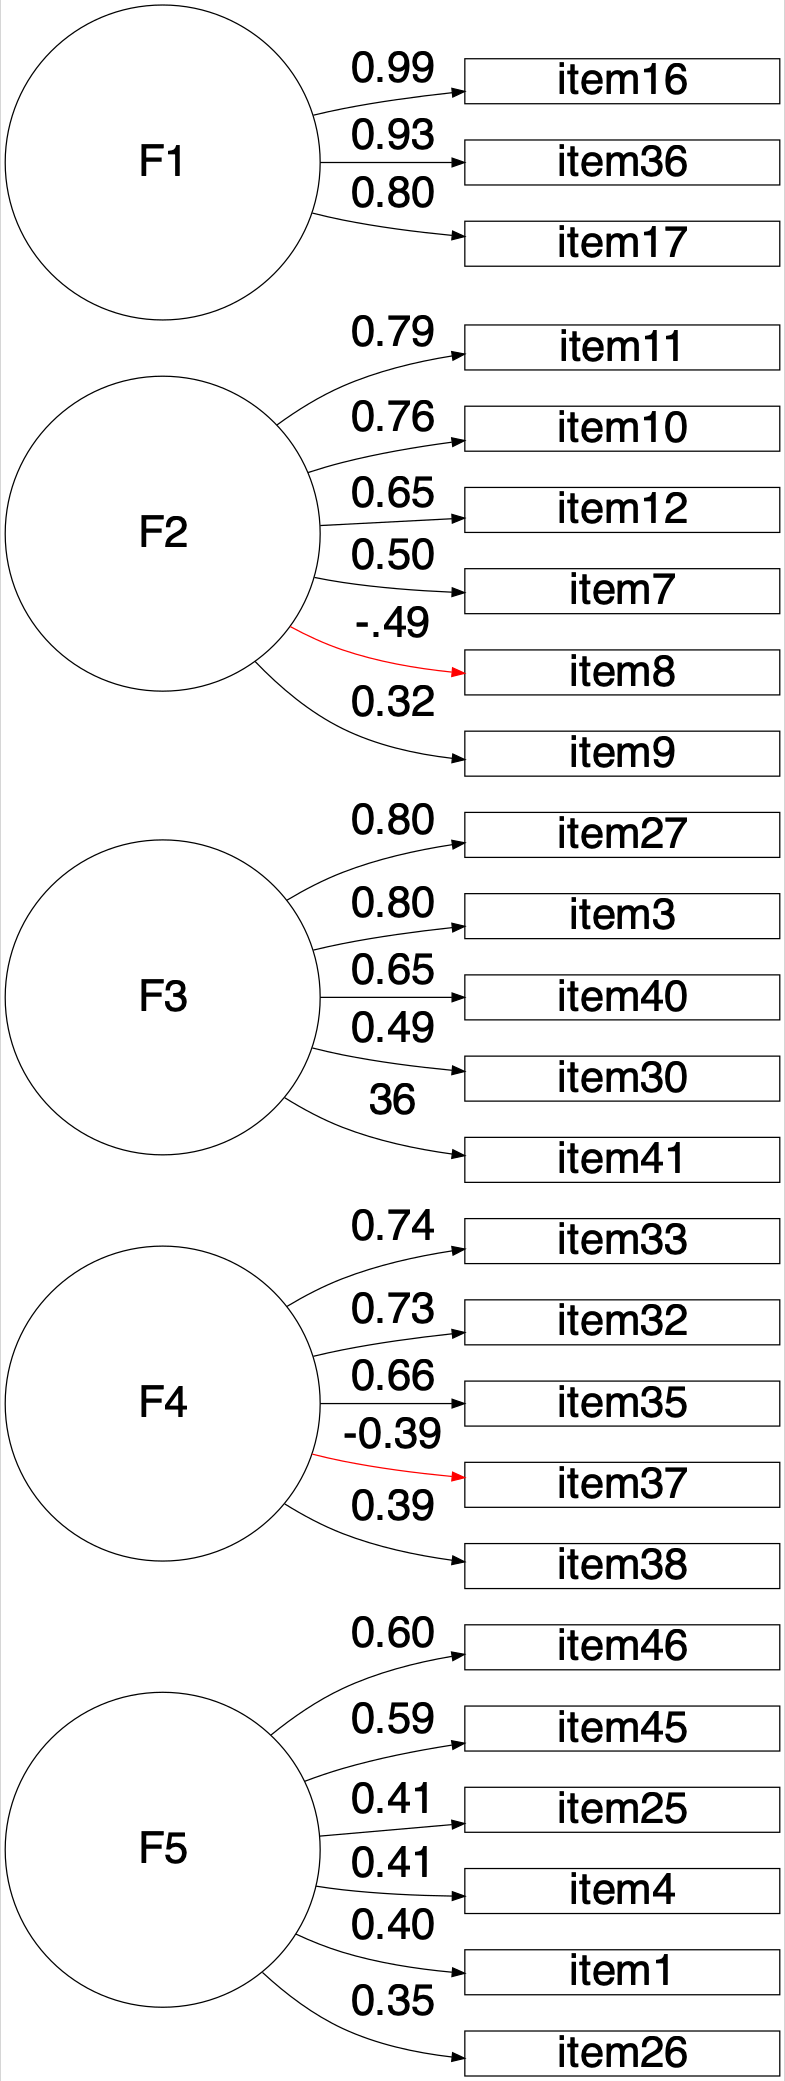
\includegraphics[width=1\linewidth,height=0.5\textheight]{Manuscript.figures/EFAplot} 

}

\caption{Five Factor Solution}\label{fig:EFAplot}
\end{figure}

With initial 48 items we conducted three rounds of EFA gradually discarded problematic items. (cross-loading items and poor factor loading (\textless.30) items). Finally, a five-factor EFA solution with 25 items was accepted with low RMSR = 0.08 (Brown, 2015), all factor-loading higher than .30 and no cross-loading greater than .30. We confirmed this five-factor latent structure using varimax rotation with a minimum residual extraction method (Table\ref{tab:MinResTab}). Table\ref{tab:EFATable} displays the factor-loading (structural coefficients) and communality of the items. The absolute value of the factor-loading ranged from -.49 to .99 indicating strong coefficients. The commonalities ranged between .11 to .99. However, the histogram of the absolute values of non-redundant residual-correlations Fig\ref{fig:EFAResiduals} showed 26\% correlations greater than the absolute value of .05, indicating a possible under-factoring. (C. D. Desjardins, 2018). Subsequently, we fitted a six-factor solution. However, a factor emerged with only one salient variable loading in the six-factor solution, thus disqualifying the six-factor solution (Table\ref{tab:sixFacTab}).

Internal consistency reliability coefficient Cronbach's alpha assumes that all the factor- loading of the items under a factor are equal (Graham, 2006; Novick \& Lewis, 1967) which is not the case in our sample. Additionally Cronbach's alpha coefficient has a tendency to deflate the estimates for Likert type data as the calculation is based on pearson-correlation matrix which requires that response data should be in continuous of nature (Gadermann, Guhn, \& Zumbo, 2012; Zumbo, Gadermann, \& Zeisser, 2007). Subsequently to get better estimates of reliability we reported ordinal alpha which used polychoric-correlation matrix and assumed that the responses data were ordered in nature instead of continuous. Ordinal alpha coefficient value ranges from 0 to 1 and higher value represents better reliability. In the five-factor solution, the first factor contained three items and explained 10.25\% of the total variance with a internal reliability coefficient ordinal \(\alpha\) = .94. All the items in this factor stemmed from the individual's preference to use blue light filters in different light environments. The second factor contained six items and explained 9.93\% of the total variance with a internal reliability coefficient ordinal \(\alpha\) = .76. Items under this factor commonly investigate an individual's hours spent outdoor. The third factor contained five items and explained 8.83\% of the total variance. Items under this factor dealt with the specific behaviors pertaining to sleep. The internal consistency reliability coefficient was, ordinal \(\alpha\) = .75. The fourth factor contained five items and explained 8.44\% of the total variance with an internal consistency coefficient, ordinal \(\alpha\) = .72. These five items stemmed from the behavior related to an individual's cellphone usage during the sleep-wakeup time. Lastly, the fifth factor contained six items and explained 6.14\% of the total variance. This factor tried to measure an individual's behavior lead by the awareness of light's influence on health. The internal consistency reliability was, ordinal \(\alpha\) = .62 . It is essential to attain a balance between psychometric properties and interpretability of the common themes when exploring the latent structure. As all of the emerged factors are highly interpretable and relevant towards our aim to capture light exposure related behavior, regardless of the apparent low reliability of the fifth factor, we retain all the five-factors with 23 items for our confirmatory factor analysis (CFA). Two items showed negative factor-loading (items 44 and 21). Upon inspection, it was understood that these items are negatively correlated to the common theme, and thus in the CFA analysis, we reversed the response code for these two items.

\begin{table}[tbp]

\begin{center}
\begin{threeparttable}

\caption{\label{tab:EFATable}Factor loadings and communality of the retained items}

\small{

\begin{tabular}{cccccccc}
\toprule
item & \multicolumn{1}{c}{PA1} & \multicolumn{1}{c}{PA2} & \multicolumn{1}{c}{PA3} & \multicolumn{1}{c}{PA4} & \multicolumn{1}{c}{PA5} & \multicolumn{1}{c}{Communality} & \multicolumn{1}{c}{Uniqueness}\\
\midrule
item16 & 0.99 &  &  &  &  & 0.993 & 0.007\\
item36 & 0.94 &  &  &  &  & 0.899 & 0.101\\
item17 & 0.8 &  &  &  &  & 0.658 & 0.342\\
item11 &  & 0.79 &  &  &  & 0.642 & 0.358\\
item10 &  & 0.76 &  &  &  & 0.592 & 0.408\\
item12 &  & 0.65 &  &  &  & 0.465 & 0.535\\
item7 &  & 0.5 &  &  &  & 0.267 & 0.733\\
item8 &  & -0.49 &  &  &  & 0.252 & 0.748\\
item9 &  & 0.32 &  &  &  & 0.113 & 0.887\\
item27 &  &  & 0.8 &  &  & 0.658 & 0.342\\
item3 &  &  & 0.8 &  &  & 0.682 & 0.318\\
item40 &  &  & 0.65 &  &  & 0.464 & 0.536\\
item30 &  &  & 0.45 &  &  & 0.353 & 0.647\\
item41 &  &  & 0.36 &  &  & 0.329 & 0.671\\
item33 &  &  &  & 0.74 &  & 0.555 & 0.445\\
item32 &  &  &  & 0.73 &  & 0.624 & 0.376\\
item35 &  &  &  & 0.66 &  & 0.454 & 0.546\\
item37 &  &  &  & -0.39 &  & 0.174 & 0.826\\
item38 &  &  &  & 0.38 &  & 0.178 & 0.822\\
item46 &  &  &  &  & 0.6 & 0.422 & 0.578\\
item45 &  &  &  &  & 0.59 & 0.374 & 0.626\\
item25 &  &  &  &  & 0.41 & 0.193 & 0.807\\
item4 &  &  &  &  & 0.41 & 0.219 & 0.781\\
item1 &  &  &  &  & 0.4 & 0.17 & 0.83\\
item26 &  &  &  &  & 0.35 & 0.165 & 0.835\\
\% of Variance & 0.1 & 0.1 & 0.09 & 0.08 & 0.06 &  & \\
\bottomrule
\addlinespace
\end{tabular}

}

\begin{tablenotes}[para]
\normalsize{\textit{Note.} Only loading higher than .30 is reported}
\end{tablenotes}

\end{threeparttable}
\end{center}

\end{table}

\begin{figure}

{\centering 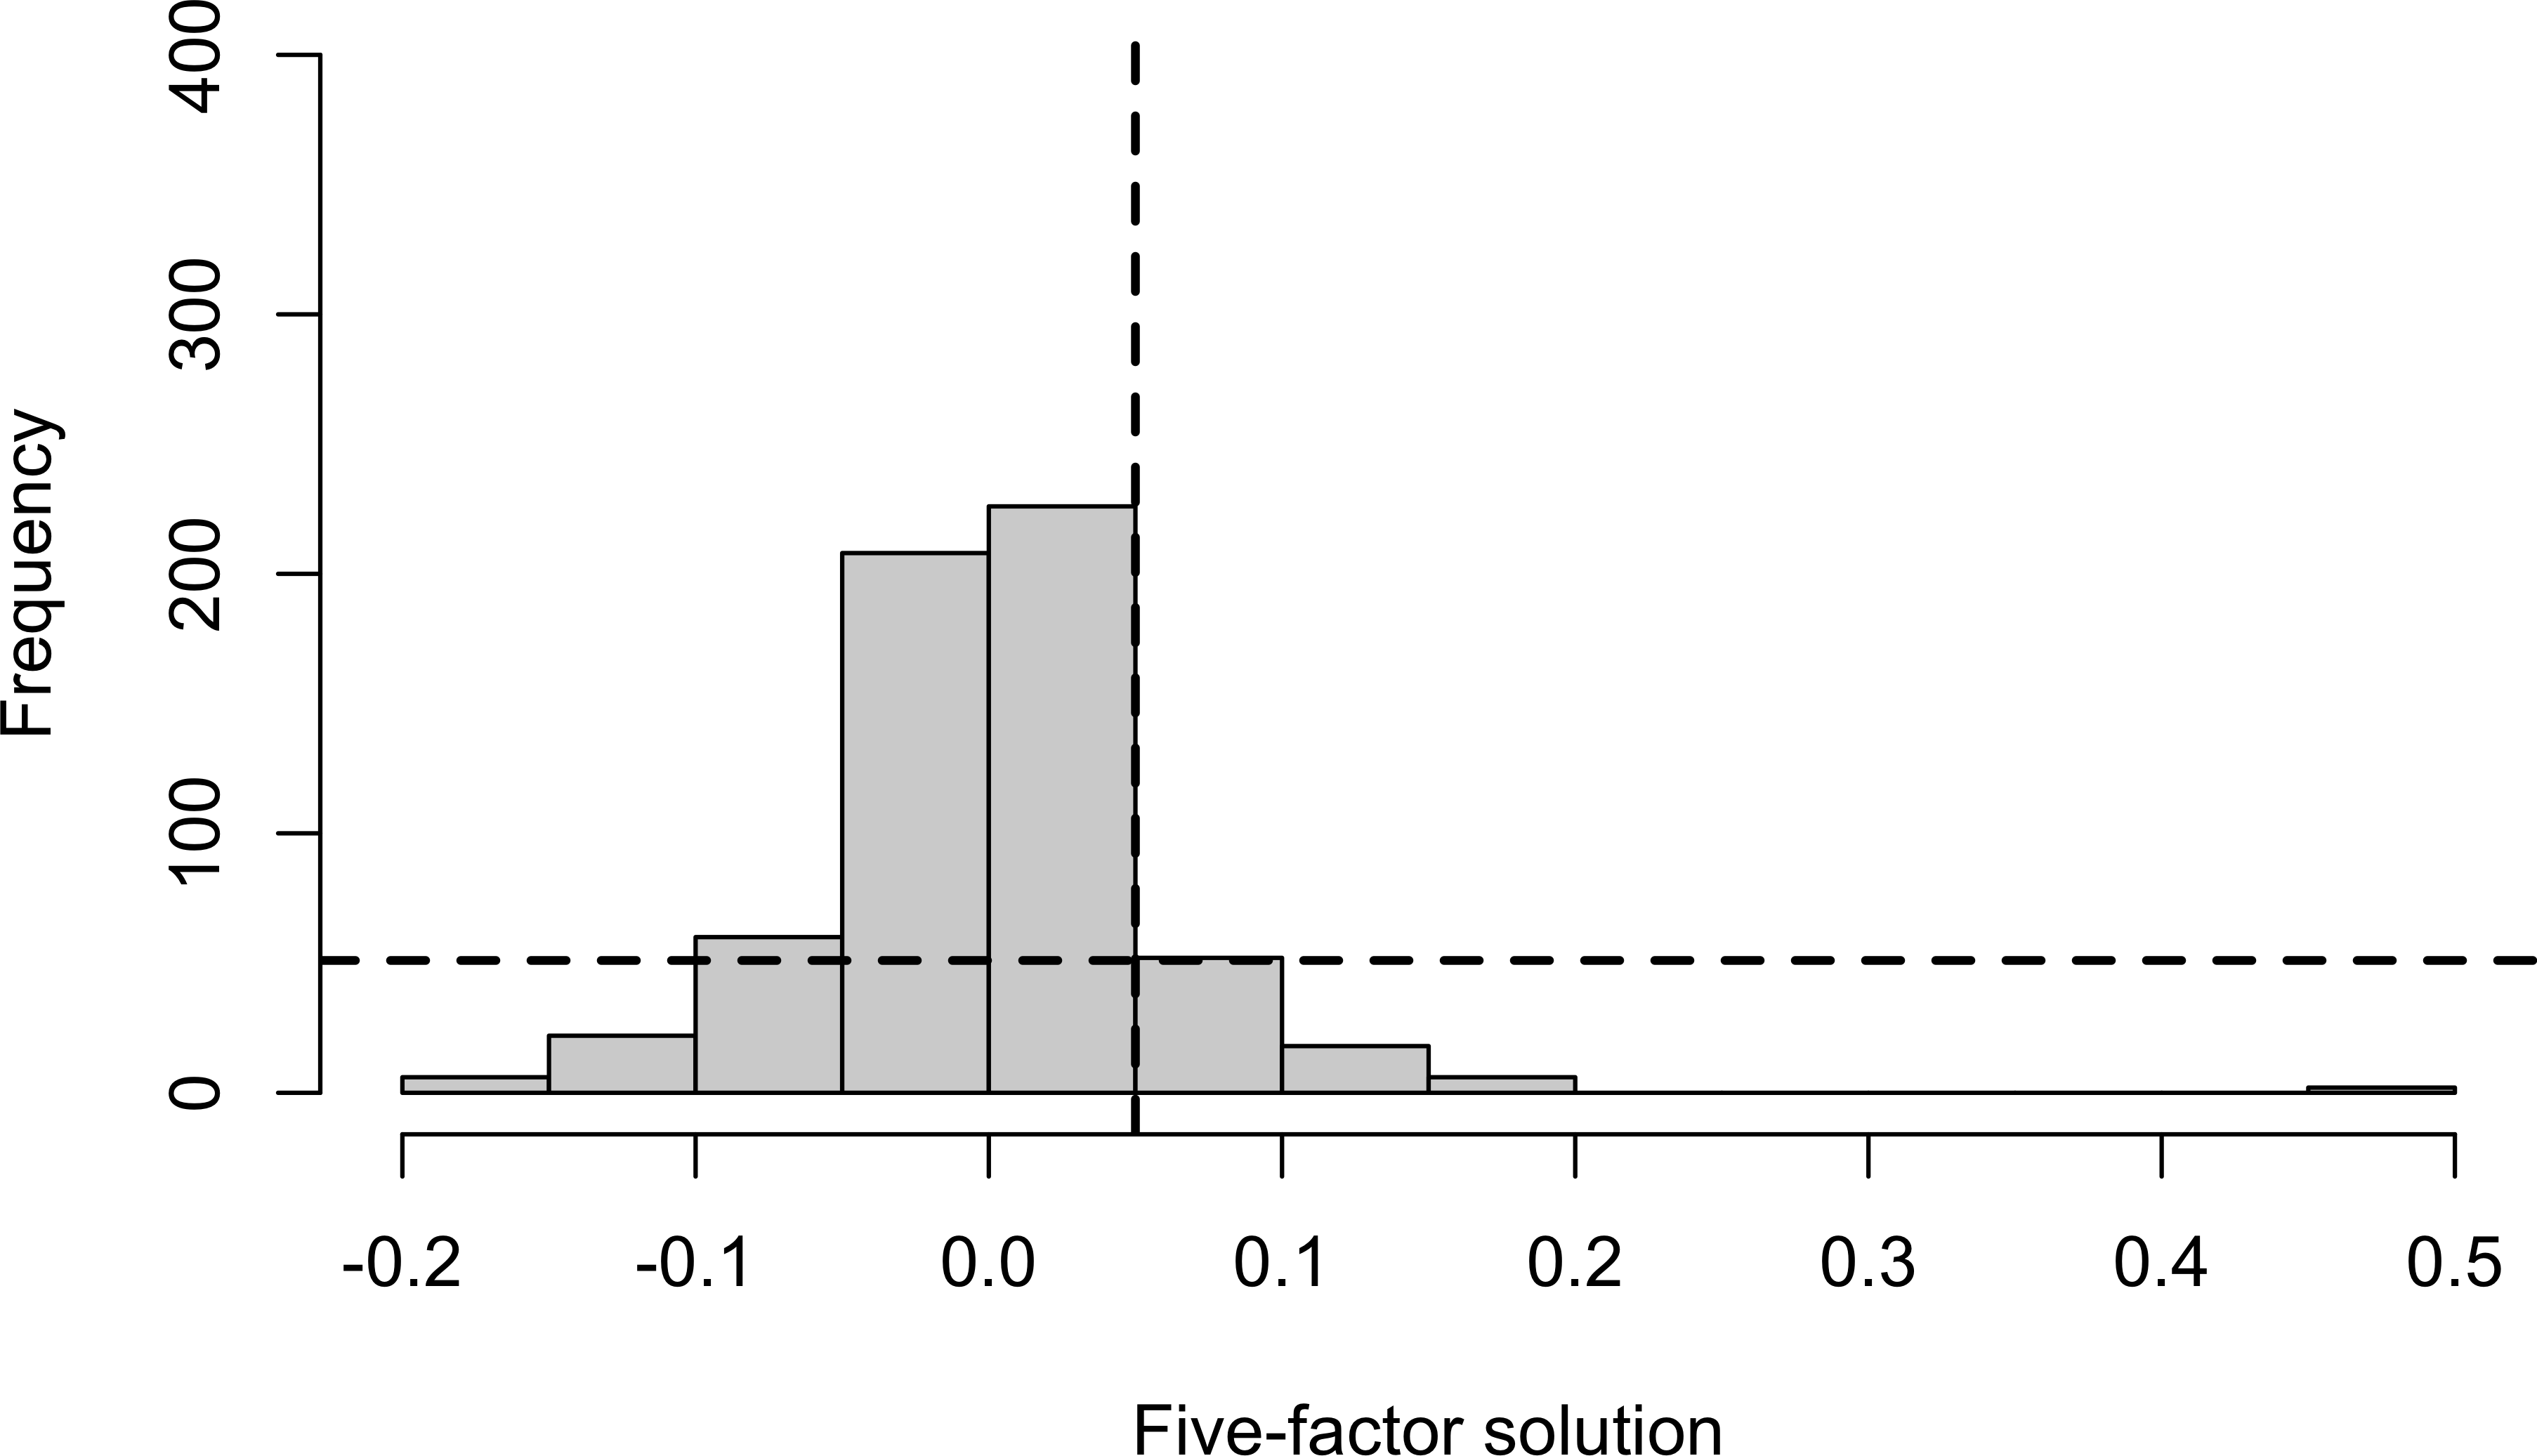
\includegraphics[width=0.5\linewidth,height=0.5\textheight]{manuscript_files/figure-latex/EFAResiduals-1} 

}

\caption{ Histogram of residulas:  five-factor solution}\label{fig:EFAResiduals}
\end{figure}

\begin{figure}
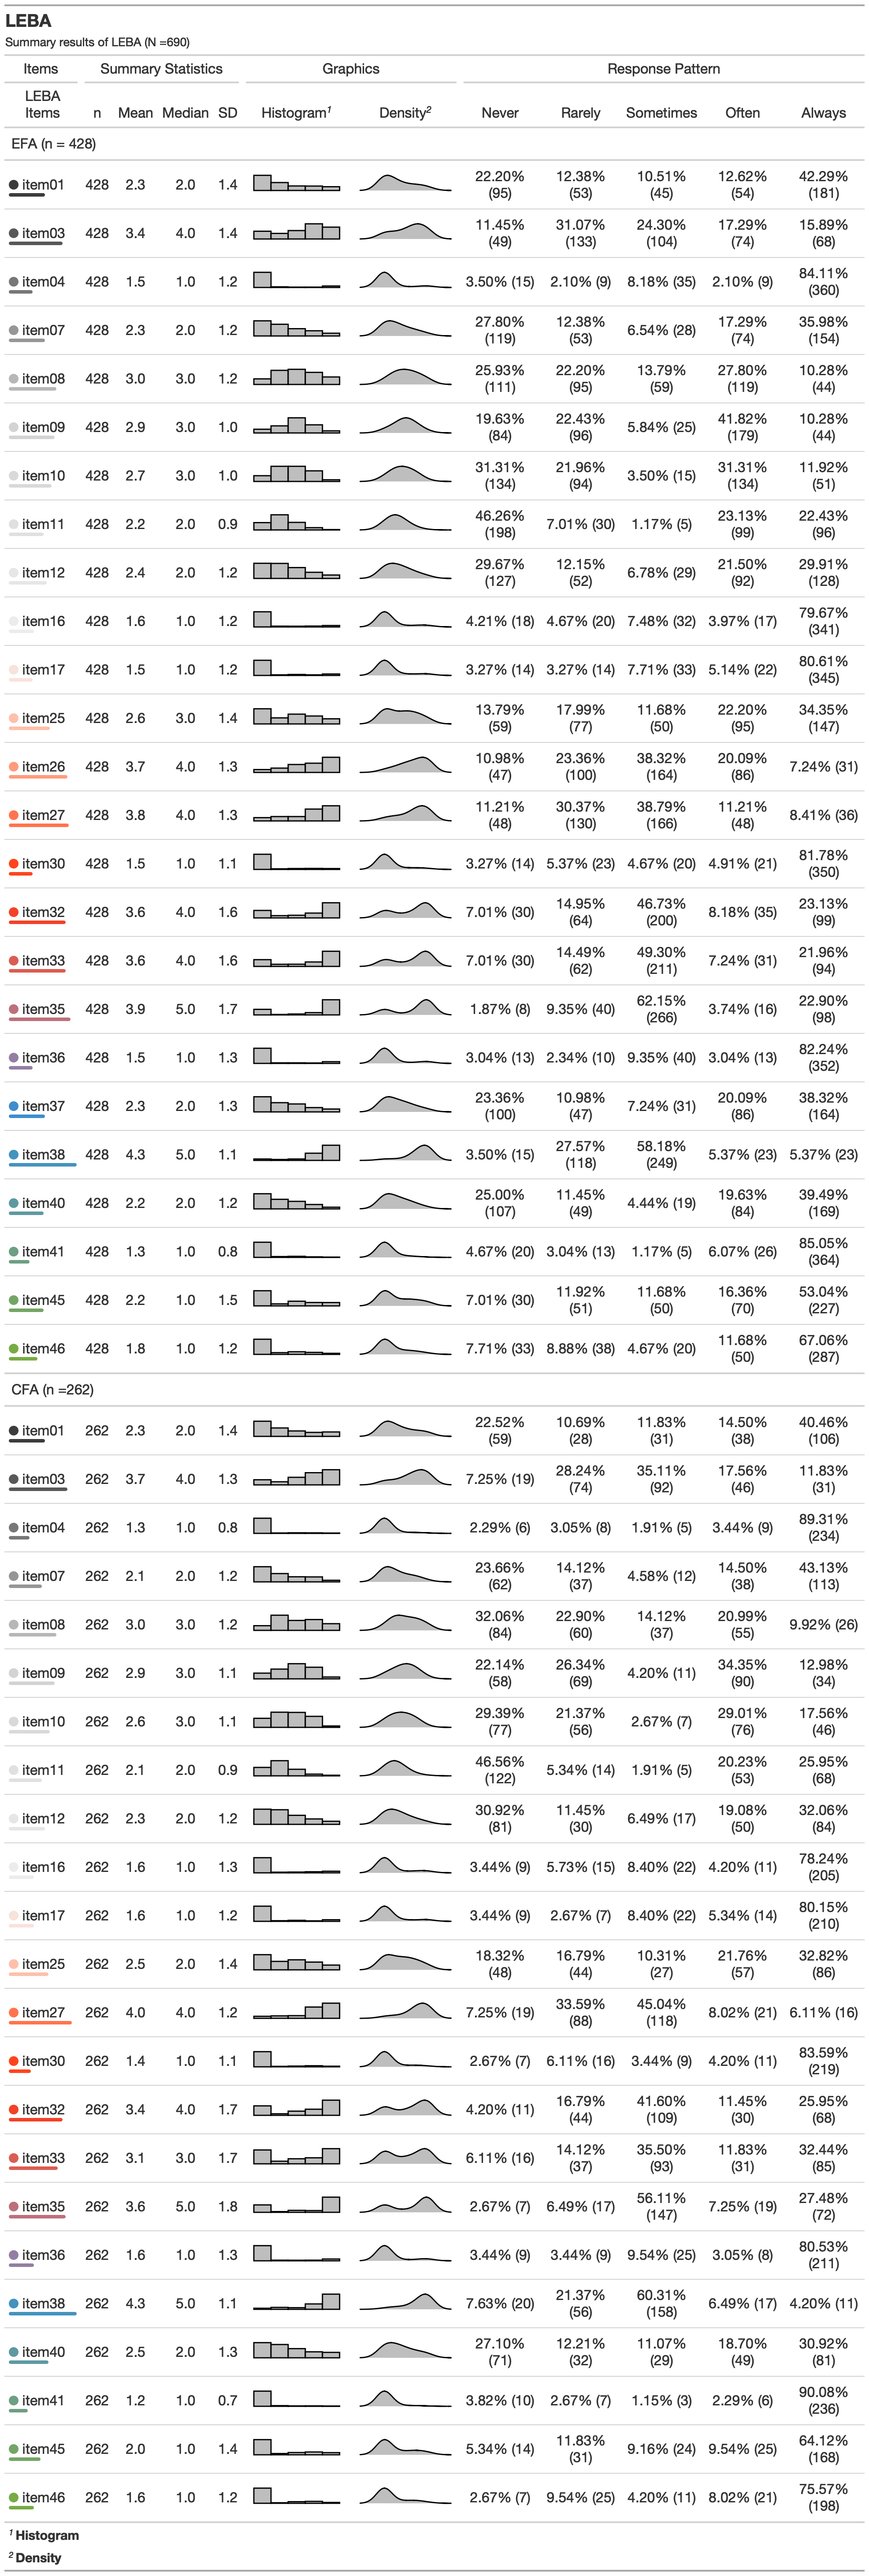
\includegraphics[width=2\linewidth,height=1\textheight]{Manuscript.figures/gt} \caption{ }\label{fig:gtPic}
\end{figure}

\hypertarget{confirmatory-factor-analysis}{%
\subsection{Confirmatory Factor Analysis}\label{confirmatory-factor-analysis}}

We conducted a categorical confirmatory factor analysis with robust weighted least square (WLSMV) estimator as our response data was in ordinary nature(C. Desjardins \& Bulut, 2018). Several indices are suggested to measure model fit. These indices can be categorized as absolute, comparative and parsimony fit indices (Brown, 2015). Absolute fit assess the model fit at an absolute level using indices including \(\chi^2\) test statistics and the standardized root mean square (SRMR).parsimony fit indices including the root mean square error of approximation (RMSEA) considers the number of free parameters in the model to assess the parsimony of the model. Comparative fit indices evaluate the fit of the specified model solution in relation to a more restricted baseline model restricting all covariances among the idicators as zero. Comparative fit index (CFI) and the Tucker Lewis index (TLI) are such two comparative fit indices. Commonly used Model fit guidelines (Hu \& Bentle, 1999; Schumacker \& Lomax, 2004) includes (i) Reporting of \(\chi^2\) test statistics (A non-significant test statistics is required to reflect model fit) (i) CFI and TLI (CFI/TLI close to .95 or above/ranging between 90-95 and above) (ii) RMSEA (close to .06 or below), (iii) SRMR (close to .08 or below) to estimate the model fit. Table \ref{tab:tabCfa} summarizes the fit indices of our fitted model. Our fitted model failed to attain an absolute fit estimated by the \(\chi^2\) test. However, the \(\chi^2\) test is sensitive to sample size and not recommended to be used as the sole index of absolute model fit (Brown, 2015). Another absolute fit index we obtained in our analysis was SRMR which does not work well with categorical data (C.-Y. Yu, 2002). Subsequently, we judged the model fit based on the comparative fit indices: CFI, TLI and parsimony fit index-RMSEA. Our fitted model attained acceptable fit (CFI =.94; TLI = .93); RMSEA = .06,{[}.05-.07, 90\% CI{]}) with two imposed equity constrain on item pairs 32-33 and 19-17 . However SRMR value was higher than the guideline (SRMR = .12). Further by allowing one pair of items (30-41) to covary their error variance and discarding two item (item 37 \& 26) for very low r-square value, our model attained best fit (CFI =.97; TLI = .96); RMSEA = .05{[}.04-.06, 90\% CI{]}) and SRMR value (SRMR = .09) was also close to the suggestions of Hu and Bentle (1999).

Internal consistency ordinal \(\alpha\) for the five factors of LEBA were .96, .83, .70, .69, .52 respectively. We also estimated the internal consistency reliability of the total scale using Mcdonald's omega(total) coefficient which is a better reliability estimate for multidimensional constructs(Dunn, Baguley, \& Brunsden, 2014; Sijtsma, 2009). McDonald's omega(total) coefficient for the total scale was .73.

\begin{lltable}

\begin{TableNotes}[para]
\normalsize{\textit{Note.} df: Degrees of Freedom; CFI: Comparative Fit Index; TLI: Tucker Lewis Index;RMSEA:Root Mean Square Error of Approximation; CI: Confidence Interval; SRMR: Standardized Root Mean Square }
\end{TableNotes}

\begin{longtable}{ccccccccc}\noalign{\getlongtablewidth\global\LTcapwidth=\longtablewidth}
\caption{\label{tab:tabCfa}Fit indices of CFA}\\
\toprule
Model & \multicolumn{1}{c}{Chi-Squre} & \multicolumn{1}{c}{df} & \multicolumn{1}{c}{CFI} & \multicolumn{1}{c}{TLI} & \multicolumn{1}{c}{RMSEA} & \multicolumn{1}{c}{RMSEA 90\% Lower CI} & \multicolumn{1}{c}{RMSEA 90\% Upper CI} & \multicolumn{1}{c}{SRMR}\\
\midrule
\endfirsthead
\caption*{\normalfont{Table \ref{tab:tabCfa} continued}}\\
\toprule
Model & \multicolumn{1}{c}{Chi-Squre} & \multicolumn{1}{c}{df} & \multicolumn{1}{c}{CFI} & \multicolumn{1}{c}{TLI} & \multicolumn{1}{c}{RMSEA} & \multicolumn{1}{c}{RMSEA 90\% Lower CI} & \multicolumn{1}{c}{RMSEA 90\% Upper CI} & \multicolumn{1}{c}{SRMR}\\
\midrule
\endhead
Five factor model:25 & 448.51 & 222.00 & .94 & 0.93 & 0.06 & 0.05 & 0.07 & 0.12\\
Five factor model:23 & 346.59 & 221.00 & .97 & 0.96 & 0.05 & 0.04 & 0.06 & 0.09\\
\bottomrule
\addlinespace
\insertTableNotes
\end{longtable}

\end{lltable}

\begin{figure}
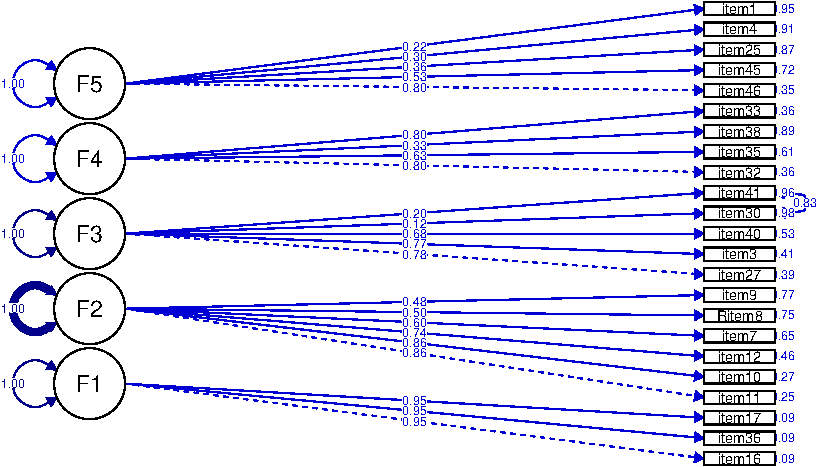
\includegraphics[width=1\linewidth]{manuscript_files/figure-latex/figcfa-1} \caption{(A) Five Factor Model of LEBA}\label{fig:figcfa}
\end{figure}

\hypertarget{measurement-invariance}{%
\section{Measurement Invariance}\label{measurement-invariance}}

Measurement invariance (MI) evaluates whether a construct has the psychometric equivalence and same meaning across groups or measurement occasions (Kline, 2015; Putnick \& Bornstein, 2016). We used structural equation modeling framework to assess measurement invariance of our developed tool across two groups: \textbf{native English speakers} and \textbf{non-native English speakers}. Our measurement invariance testing involved establishing configural, metric , scalar , and residual invariance (Widaman \& Reise, 1997). MI models are nested type models of which configural model is the first and least restrictive model. Configural model assumes that the number of factors and item number under each factors will be equal across two groups. Metric invariance model along with the assumption of configural model assumes that factor-loadings of the items across the two groups will be equal indicating each item contributes to the measured construct equivalently for the both groups. Along with these assumptions scalar invariance assumes that item intercepts to be equivalent across groups. Scalar invariance model indicates the equivalence of response scale across the groups, i.e.~persons with the same level of the underlying construct will score the same across the groups. Residual invariance model holds all the mentioned assumptions as true and also adds the assumption of equality in error variances and covariances across the groups. This model is the highest level of MI and assures the equivalence of precision of items across the groups in measuring the underlying constructs. The invariance model fit was assessed using the fit indices including \(\chi^2\) test, CFI and TLI (close to .95 or above) , RMSEA (close to .06 or below). following the guidelines of Hu and Bentle (1999). We excluded SRMR from our consideration as it does not behave optimally for categorical variables (C.-Y. Yu, 2002). Table \ref{tab:InvarianceTab} summarized the fit indices. The comparison among different measurement invariance model was made by using \(\chi^2\) difference test (\(\Delta \chi^2\)) to assess whether our obtained latent structure of ``LEBA'' attains the highest level of the MI. If the \(\Delta \chi^2\) is not statistically significant (p\textless0.05) (Dimitrov, 2010) the particular invariance model was accepted. We started our analysis by comparing the model fit of the lest restrictive model:configural model to metric MI model and continued successive comparisons. Table \ref{tab:InvarianceTab} indicates that our fiited model attains residual invariance: the highest level of invariance in terms of CFI, TLI, RMSEA and non-significant \(\Delta \chi^2\) test.

\begin{lltable}

\begin{TableNotes}[para]
\normalsize{\textit{Note.}  a = Metric vs Configural; b = Scalar vs Metric; c = Residual vs Scalar; d = Structural vs Residual;* =  df of model comparison}
\end{TableNotes}

\footnotesize{

\begin{longtable}{ccccccccccc}\noalign{\getlongtablewidth\global\LTcapwidth=\longtablewidth}
\caption{\label{tab:InvarianceTab}Invariance Analysis}\\
\toprule
 & \multicolumn{1}{c}{Chi-Square} & \multicolumn{1}{c}{df} & \multicolumn{1}{c}{CFI} & \multicolumn{1}{c}{TLI} & \multicolumn{1}{c}{RMSEA} & \multicolumn{1}{c}{RMSEA 90\% Lower CI} & \multicolumn{1}{c}{RMSEA 90\% Upper} & \multicolumn{1}{c}{Chi-Square Difference} & \multicolumn{1}{c}{df difference*} & \multicolumn{1}{c}{p}\\
\midrule
\endfirsthead
\caption*{\normalfont{Table \ref{tab:InvarianceTab} continued}}\\
\toprule
 & \multicolumn{1}{c}{Chi-Square} & \multicolumn{1}{c}{df} & \multicolumn{1}{c}{CFI} & \multicolumn{1}{c}{TLI} & \multicolumn{1}{c}{RMSEA} & \multicolumn{1}{c}{RMSEA 90\% Lower CI} & \multicolumn{1}{c}{RMSEA 90\% Upper} & \multicolumn{1}{c}{Chi-Square Difference} & \multicolumn{1}{c}{df difference*} & \multicolumn{1}{c}{p}\\
\midrule
\endhead
Configural & 632.20 & 442.00 & 0.95 & 0.94 & 0.06 & 0.05 & 0.07 & - & - & -\\
Metric & 644.58 & 458.00 & 0.95 & 0.95 & 0.06 & 0.05 & 0.07 & 18.019a & 16 & 0.323\\
Scalar & 714.19 & 522.00 & 0.95 & 0.95 & 0.05 & 0.04 & 0.06 & 67.961b & 64 & 0.344\\
Residual & 714.19 & 522.00 & 0.95 & 0.95 & 0.05 & 0.04 & 0.06 & 0c & 0 & NA\\
\bottomrule
\addlinespace
\insertTableNotes
\end{longtable}

}

\end{lltable}

\hypertarget{analysing-the-quality-of-items-by-item-information-theory}{%
\subsection{Analysing the quality of items by Item Information Theory}\label{analysing-the-quality-of-items-by-item-information-theory}}

We sought the IRT to gether information regarding the item quality. IRT complements the conventional classical test theory-based analysis by gathering information on item discrimination and item difficulty(Baker, 2017). Here, an item's quality is judged based on item information in relation to participants' latent trait level (\(\theta\)). We gathered evidence on item quality by fitting each factor of LEBA with the graded response model (\ref{tab:IRTparameters} to the combined EFA sample and CFA sample (n =690). Item discrimination indicates the pattern of variation in the categorical responses with the changes in latent trait, and item information curve (IIC) indicates the amount of information an item carries along the latent trait continuum. Here, we reported the item discrimination parameter and only discarded the items with relatively flat item information curve (information \textless.2) to develop the short form of LEBA. Baker (2017) categorized the item discrimination in as none = 0; very low =0.01 to 0.34; low = 0.35 to 0.64; moderate = 0.65 to 1.34 ; high = 1.35 to 1.69; very high \textgreater1.70. Item discrimination parameters of our scale fell in very high (10 items), high (4 items), moderate (4 items), low ( 5 items) indicating a good range of discrimination along the latent trait. Examination of the item information curve indicated 6 items (1, 25, 9, 38, 30, \& 41) had relatively flat information curves thus discarded. We also gathered evidence of item fit and person fit to our fitted model.

\begin{table}[tbp]

\begin{center}
\begin{threeparttable}

\caption{\label{tab:IRTparameters}IRT Item parameters for the LEBA Scale}

\begin{tabular}{llllll}
\toprule
 & \multicolumn{1}{c}{a} & \multicolumn{1}{c}{b1} & \multicolumn{1}{c}{b2} & \multicolumn{1}{c}{b3} & \multicolumn{1}{c}{b4}\\
\midrule
item16 & 28.55 & 0.78 & 0.90 & 1.06 & 1.40\\
item36 & 4.49 & 0.94 & 1.08 & 1.23 & 1.40\\
item17 & 2.81 & 0.97 & 1.11 & 1.38 & 1.62\\
item11 & 3.27 & -0.79 & 0.65 & 1.54 & 2.31\\
item10 & 3.07 & -1.27 & -0.09 & 0.82 & 2.00\\
item12 & 1.72 & -0.67 & 0.44 & 1.28 & 2.11\\
item7 & 1.09 & -0.50 & 0.73 & 1.63 & 2.97\\
Ritem8 & 1.19 & -2.26 & -0.48 & 0.64 & 1.91\\
item9 & 0.91 & -2.63 & -0.96 & 1.11 & 3.49\\
item27 & 2.21 & -1.88 & -1.19 & -0.73 & 0.30\\
item3 & 3.03 & -1.24 & -0.77 & -0.20 & 0.66\\
item40 & 1.55 & -0.51 & 0.46 & 1.32 & 2.22\\
item30 & 0.49 & 3.27 & 3.74 & 4.64 & 6.52\\
item41 & 0.51 & 3.87 & 4.78 & 6.39 & 8.91\\
item32 & 1.62 & -1.03 & -0.78 & -0.42 & 0.16\\
item35 & 1.36 & -1.09 & -0.98 & -0.75 & -0.40\\
item38 & 0.40 & -7.50 & -5.58 & -4.25 & -0.91\\
item33 & 13.51 & -0.66 & -0.48 & -0.24 & 0.13\\
item46 & 2.22 & 0.68 & 0.89 & 1.38 & 2.17\\
item45 & 1.51 & 0.30 & 0.55 & 1.17 & 1.91\\
item25 & 0.52 & -1.37 & -0.04 & 1.89 & 4.22\\
item4 & 0.84 & 2.44 & 2.80 & 3.18 & 3.67\\
item1 & 0.39 & -0.91 & 1.52 & 3.25 & 5.53\\
\bottomrule
\addlinespace
\end{tabular}

\begin{tablenotes}[para]
\normalsize{\textit{Note.} a = item discrimination parameter; b(1-4) = response category difficulty parameter}
\end{tablenotes}

\end{threeparttable}
\end{center}

\end{table}

\begin{figure}
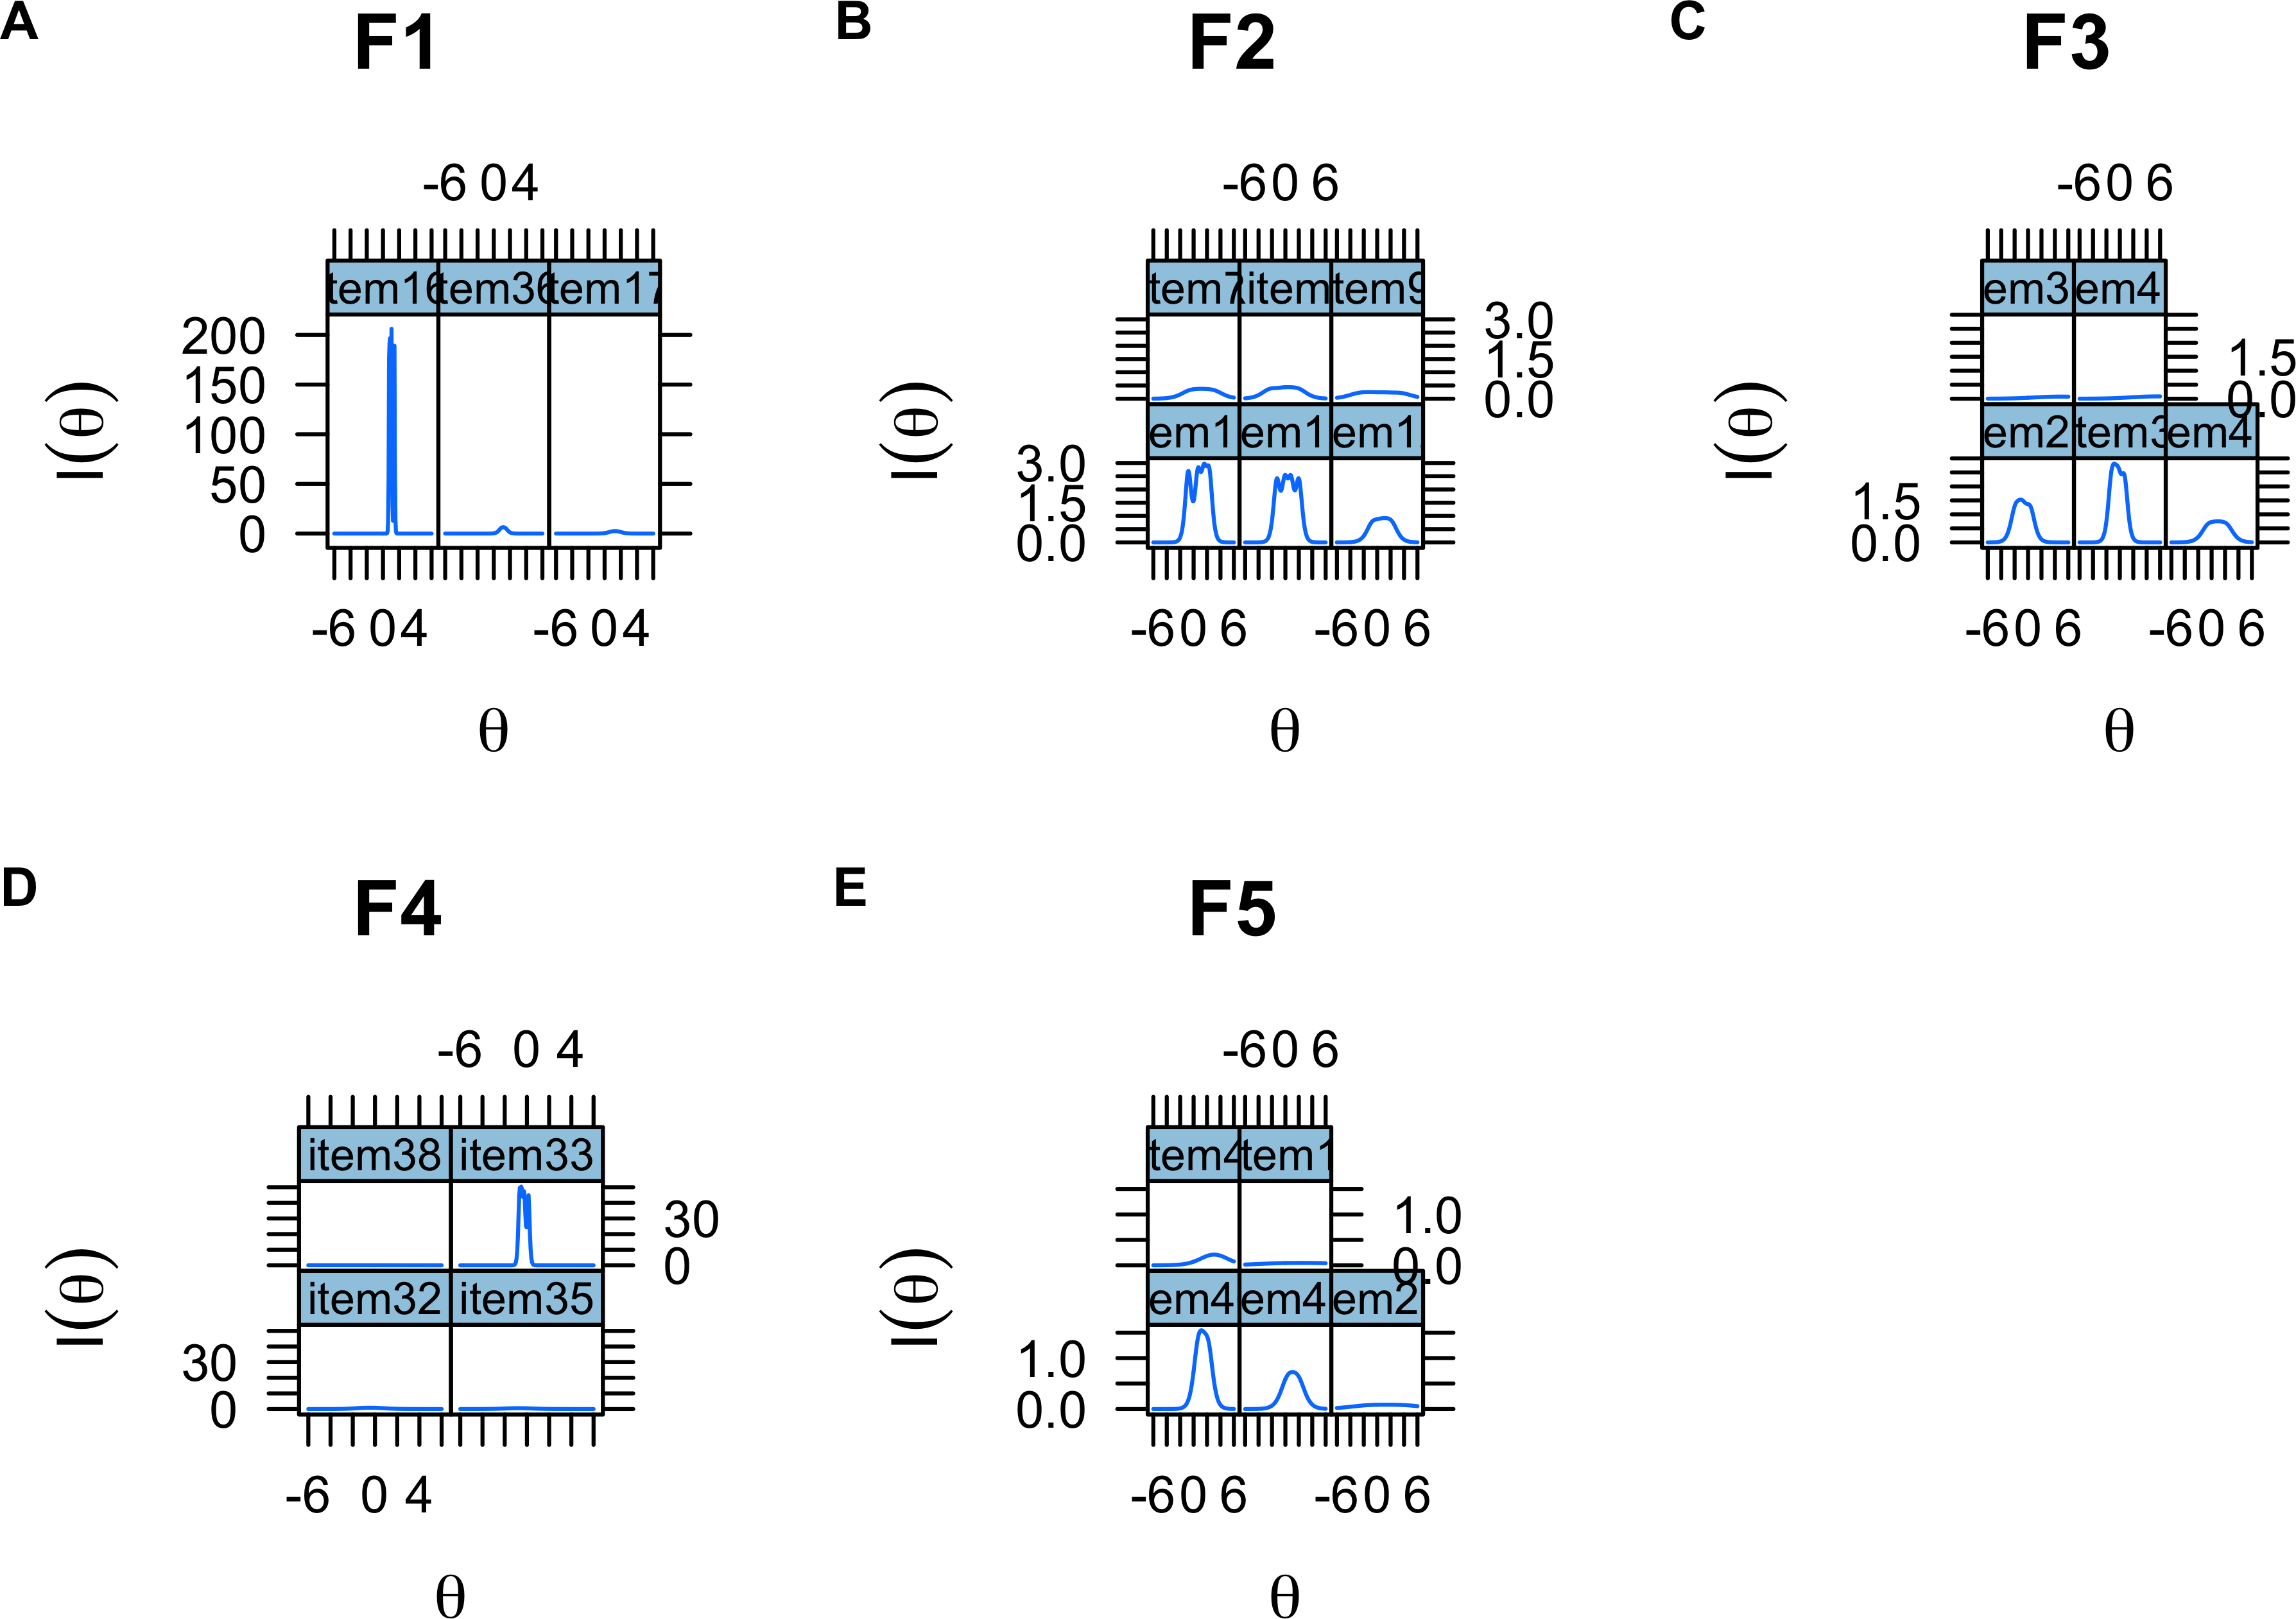
\includegraphics[width=1\linewidth,height=1.2\textheight]{manuscript_files/figure-latex/itmeinfo-1} \caption{Item information curves (A) blue filter (B) natural light (C)smart device (D)sleep environment (E)electic light}\label{fig:itmeinfo}
\end{figure}

\begin{figure}
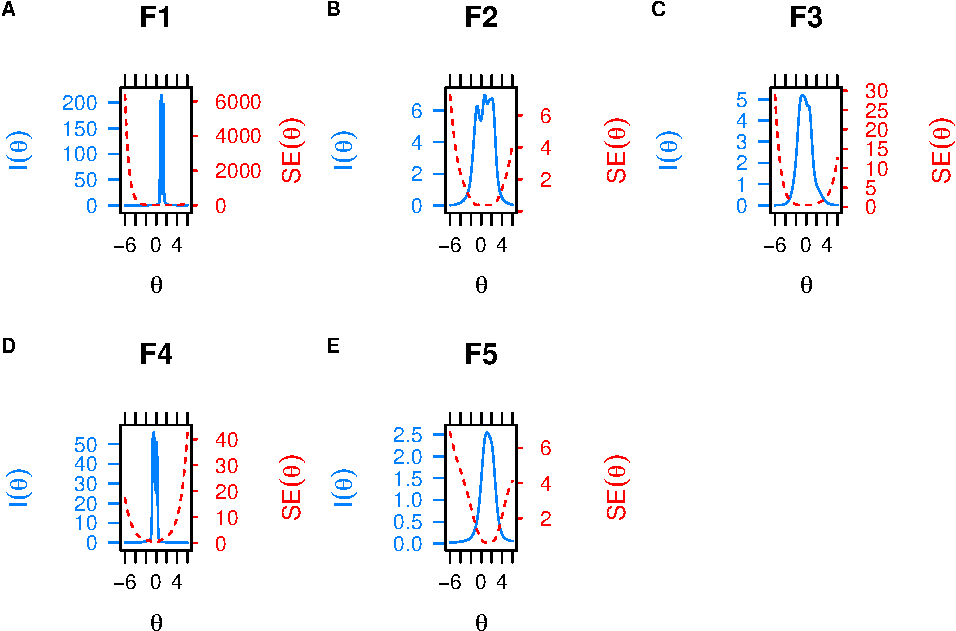
\includegraphics[width=1\linewidth,height=1.2\textheight]{manuscript_files/figure-latex/Testinfo-1} \caption{Test information curves (A) blue filter (B) natural light (C)smart device (D)sleep environment (E)electic light}\label{fig:Testinfo}
\end{figure}

Test information curve (TIC) indicate the amount of information an the full-scale carry along the latent trait continuum. As we treated each factor of LEBA as an unidmensional construct we obtain 5 TICs. These information curves indicated except blue filter factor, the other factor's TICs are roughly centered on the center of the trait continuum ((\(\theta\))). Also the amount of information changed rather steadily with the change of (\(\theta\)). Thus we conferred the LEBA scale (except blue filter) estimated the light exposure related behavior with precision near the center of trait continuum (Baker, 2017) which is sufficient to discriminate between latent trait measured by the each factor. The blue filter factor had a peak to the right side of the center of latent trait indicating its ability to providing information only for people who already have some preference towards using blue-filters.

Our result also indicated all the items fitted well to the respective models as assessed by assessed by RMSEA value obtained from Signed-X2 index implementation. All of the items had RMSEA value \textless.06 indicating adequate fit. Person fit indicates the validity and meaningfulness of the fitted model at the participants latent trait level (C. Desjardins \& Bulut, 2018). We estimated the person fit statistics using standardized fit index Zh statistics (Drasgow, Levine, \& Williams, 1985). Zh \textless{} -2 should be considered as a misfit. Fig indicates that Zh is larger than -2 for most participants, suggesting a good fit of the selected IRT models.

The overall we can concluded that IRT analysis indicated LEBA is a psychometrically sound measure. Item fit indexes and person fit index for all five fitted model were acceptable. Items had diverse slope parameters indicating a good range of discrimination- the ability to differentiate respondents with different levels of the light exposure related behavior. All-in-all we can recommend the LEBA to be used to capture light exposure related behavior.

\hypertarget{discussion}{%
\section{Discussion}\label{discussion}}

\newpage

\hypertarget{references}{%
\section{References}\label{references}}

\begingroup
\setlength{\parindent}{-0.5in}
\setlength{\leftskip}{0.5in}

\hypertarget{refs}{}
\begin{CSLReferences}{1}{0}
\leavevmode\vadjust pre{\hypertarget{ref-R-tabledown}{}}%
Anwar Siraji, M. (2021). \emph{Tabledown: A companion pack for the book "basic \& advanced psychometrics in r"}. Retrieved from \url{https://github.com/masiraji/tabledown}

\leavevmode\vadjust pre{\hypertarget{ref-R-papaja}{}}%
Aust, F., \& Barth, M. (2020). \emph{{papaja}: {Prepare} reproducible {APA} journal articles with {R Markdown}}. Retrieved from \url{https://github.com/crsh/papaja}

\leavevmode\vadjust pre{\hypertarget{ref-bajaj2011validation}{}}%
Bajaj, A., Rosner, B., Lockley, S. W., \& Schernhammer, E. S. (2011). Validation of a light questionnaire with real-life photopic illuminance measurements: The harvard light exposure assessment questionnaire. \emph{Cancer Epidemiology and Prevention Biomarkers}, \emph{20}(7), 1341--1349.

\leavevmode\vadjust pre{\hypertarget{ref-bakerBasicsItemResponse2017}{}}%
Baker, F. B. (2017). \emph{The {Basics} of {Item Response Theory Using R}} (1st ed. 2017.). {Springer}.

\leavevmode\vadjust pre{\hypertarget{ref-bandalosFactorAnalysisExploratory2018}{}}%
Bandalos, D. L., \& Finney, S. J. (2018). Factor analysis: {Exploratory} and confirmatory. In \emph{The reviewer's guide to quantitative methods in the social sciences} (pp. 98--122). {Routledge}.

\leavevmode\vadjust pre{\hypertarget{ref-R-questionr}{}}%
Barnier, J., Briatte, F., \& Larmarange, J. (2020). \emph{Questionr: Functions to make surveys processing easier}. Retrieved from \url{https://CRAN.R-project.org/package=questionr}

\leavevmode\vadjust pre{\hypertarget{ref-R-tinylabels}{}}%
Barth, M. (2021). \emph{{tinylabels}: Lightweight variable labels}. Retrieved from \url{https://github.com/mariusbarth/tinylabels}

\leavevmode\vadjust pre{\hypertarget{ref-bartlettNoteMultiplyingFactors1954}{}}%
Bartlett, M. (1954). A {Note} on the {Multiplying Factors} for {Various Chi}-square {Approximations}. \emph{Journal of the Royal Statistical Society. Series B, Methodological}, \emph{16}(2), 296--298.

\leavevmode\vadjust pre{\hypertarget{ref-bentlerPracticalIssuesStructural1987}{}}%
Bentler, P. M., \& Chou, C.-P. (1987). Practical {Issues} in {Structural Modeling}. \emph{Sociological Methods \& Research}, \emph{16}(1), 78--117. \url{https://doi.org/10.1177/0049124187016001004}

\leavevmode\vadjust pre{\hypertarget{ref-Bevans.2019}{}}%
Bevans, K. B., Meltzer, L. J., La Motte, A. de, Kratchman, A., Viél, D., \& Forrest, C. B. (2019). Qualitative development and content validation of the PROMIS pediatric sleep health items. \emph{Behavioral Sleep Medicine}, \emph{17}(5), 657--671. \url{https://doi.org/10.1080/15402002.2018.1461102}

\leavevmode\vadjust pre{\hypertarget{ref-brownConfirmatoryFactorAnalysis2015}{}}%
Brown, T. A. (2015). \emph{Confirmatory factor analysis for applied research} (2nd ed.). {New York, NY, US}: {The Guilford Press}.

\leavevmode\vadjust pre{\hypertarget{ref-R-likert}{}}%
Bryer, J., \& Speerschneider, K. (2016). \emph{Likert: Analysis and visualization likert items}. Retrieved from \url{https://CRAN.R-project.org/package=likert}

\leavevmode\vadjust pre{\hypertarget{ref-R-MOTE}{}}%
Buchanan, E. M., Gillenwaters, A., Scofield, J. E., \& Valentine, K. D. (2019). \emph{{MOTE: Measure of the Effect}: Package to assist in effect size calculations and their confidence intervals}. Retrieved from \url{http://github.com/doomlab/MOTE}

\leavevmode\vadjust pre{\hypertarget{ref-buysse1989pittsburgh}{}}%
Buysse, Daniel J., Reynolds III, C. F., Monk, T. H., Berman, S. R., \& Kupfer, D. J. (1989). The pittsburgh sleep quality index: A new instrument for psychiatric practice and research. \emph{Psychiatry Research}, \emph{28}(2), 193--213.

\leavevmode\vadjust pre{\hypertarget{ref-Buysse.2010}{}}%
Buysse, Daniel J., Yu, L., Moul, D. E., Germain, A., Stover, A., Dodds, N. E., \ldots{} Pilkonis, P. A. (2010). Development and validation of patient-reported outcome measures for sleep disturbance and sleep-related impairments. \emph{Sleep}, \emph{33}(6), 781--792. \url{https://doi.org/10.1093/sleep/33.6.781}

\leavevmode\vadjust pre{\hypertarget{ref-cattellScreeTestNumber1966}{}}%
Cattell, R. B. (1966). The {Scree Test For The Number Of Factors}. \emph{Multivariate Behavioral Research}, \emph{1}(2), 245--276. \url{https://doi.org/10.1207/s15327906mbr0102_10}

\leavevmode\vadjust pre{\hypertarget{ref-R-mirt}{}}%
Chalmers, R. P. (2012). {mirt}: A multidimensional item response theory package for the {R} environment. \emph{Journal of Statistical Software}, \emph{48}(6), 1--29. \url{https://doi.org/10.18637/jss.v048.i06}

\leavevmode\vadjust pre{\hypertarget{ref-R-shiny}{}}%
Chang, W., Cheng, J., Allaire, J., Sievert, C., Schloerke, B., Xie, Y., \ldots{} Borges, B. (2021). \emph{Shiny: Web application framework for r}. Retrieved from \url{https://CRAN.R-project.org/package=shiny}

\leavevmode\vadjust pre{\hypertarget{ref-comreyFirstCourseFactor1992}{}}%
Comrey, A. L., \& Lee, H. B. (1992). \emph{A first course in factor analysis, 2nd ed}. {Hillsdale, NJ, US}: {Lawrence Erlbaum Associates, Inc}.

\leavevmode\vadjust pre{\hypertarget{ref-R-corx}{}}%
Conigrave, J. (2020). \emph{Corx: Create and format correlation matrices}. Retrieved from \url{https://CRAN.R-project.org/package=corx}

\leavevmode\vadjust pre{\hypertarget{ref-R-xtable}{}}%
Dahl, D. B., Scott, D., Roosen, C., Magnusson, A., \& Swinton, J. (2019). \emph{Xtable: Export tables to LaTeX or HTML}. Retrieved from \url{https://CRAN.R-project.org/package=xtable}

\leavevmode\vadjust pre{\hypertarget{ref-desjardinsHandbookEducationalMeasurement2018a}{}}%
Desjardins, C. D. (2018). \emph{Handbook of educational measurement and psychometrics using {R}}. (O. Bulut \& ProQuest (Firm), Eds.). {Boca Raton, FL : CRC Press}.

\leavevmode\vadjust pre{\hypertarget{ref-desjardinsHandbookEducationalMeasurement2018}{}}%
Desjardins, C., \& Bulut, O. (2018). \emph{Handbook of {Educational Measurement} and {Psychometrics Using R}}. \url{https://doi.org/10.1201/b20498}

\leavevmode\vadjust pre{\hypertarget{ref-dianat2013objective}{}}%
Dianat, I., Sedghi, A., Bagherzade, J., Jafarabadi, M. A., \& Stedmon, A. W. (2013). Objective and subjective assessments of lighting in a hospital setting: Implications for health, safety and performance. \emph{Ergonomics}, \emph{56}(10), 1535--1545.

\leavevmode\vadjust pre{\hypertarget{ref-dimitrov2010testing}{}}%
Dimitrov, D. M. (2010). Testing for factorial invariance in the context of construct validation. \emph{Measurement and Evaluation in Counseling and Development}, \emph{43}(2), 121--149.

\leavevmode\vadjust pre{\hypertarget{ref-R-paran}{}}%
Dinno, A. (2018). \emph{Paran: Horn's test of principal components/factors}. Retrieved from \url{https://CRAN.R-project.org/package=paran}

\leavevmode\vadjust pre{\hypertarget{ref-drasgow1985appropriateness}{}}%
Drasgow, F., Levine, M. V., \& Williams, E. A. (1985). Appropriateness measurement with polychotomous item response models and standardized indices. \emph{British Journal of Mathematical and Statistical Psychology}, \emph{38}(1), 67--86.

\leavevmode\vadjust pre{\hypertarget{ref-dunn2014alpha}{}}%
Dunn, T. J., Baguley, T., \& Brunsden, V. (2014). From alpha to omega: A practical solution to the pervasive problem of internal consistency estimation. \emph{British Journal of Psychology}, \emph{105}(3), 399--412.

\leavevmode\vadjust pre{\hypertarget{ref-eklund1996development}{}}%
Eklund, N., \& Boyce, P. (1996). The development of a reliable, valid, and simple office lighting survey. \emph{Journal of the Illuminating Engineering Society}, \emph{25}(2), 25--40.

\leavevmode\vadjust pre{\hypertarget{ref-R-semPlot}{}}%
Epskamp, S. (2019). \emph{semPlot: Path diagrams and visual analysis of various SEM packages' output}. Retrieved from \url{https://CRAN.R-project.org/package=semPlot}

\leavevmode\vadjust pre{\hypertarget{ref-R-qgraph}{}}%
Epskamp, S., Cramer, A. O. J., Waldorp, L. J., Schmittmann, V. D., \& Borsboom, D. (2012). {qgraph}: Network visualizations of relationships in psychometric data. \emph{Journal of Statistical Software}, \emph{48}(4), 1--18.

\leavevmode\vadjust pre{\hypertarget{ref-f.lux}{}}%
F.lux Software LLC. (2021). F.lux (Version 4.120). Retrieved from \url{https://justgetflux.com/}

\leavevmode\vadjust pre{\hypertarget{ref-Forrest.2018}{}}%
Forrest, C. B., Meltzer, L. J., Marcus, C. L., La Motte, A. de, Kratchman, A., Buysse, D. J., \ldots{} Bevans, K. B. (2018). Development and validation of the PROMIS pediatric sleep disturbance and sleep-related impairment item banks. \emph{Sleep}, \emph{41}(6). \url{https://doi.org/10.1093/sleep/zsy054}

\leavevmode\vadjust pre{\hypertarget{ref-R-car}{}}%
Fox, J., \& Weisberg, S. (2019). \emph{An {R} companion to applied regression} (Third). Thousand Oaks {CA}: Sage. Retrieved from \url{https://socialsciences.mcmaster.ca/jfox/Books/Companion/}

\leavevmode\vadjust pre{\hypertarget{ref-R-carData}{}}%
Fox, J., Weisberg, S., \& Price, B. (2020). \emph{carData: Companion to applied regression data sets}. Retrieved from \url{https://CRAN.R-project.org/package=carData}

\leavevmode\vadjust pre{\hypertarget{ref-gadermann2012estimating}{}}%
Gadermann, A. M., Guhn, M., \& Zumbo, B. D. (2012). Estimating ordinal reliability for likert-type and ordinal item response data: A conceptual, empirical, and practical guide. \emph{Practical Assessment, Research, and Evaluation}, \emph{17}(1), 3.

\leavevmode\vadjust pre{\hypertarget{ref-graham2006congeneric}{}}%
Graham, J. M. (2006). Congeneric and (essentially) tau-equivalent estimates of score reliability: What they are and how to use them. \emph{Educational and Psychological Measurement}, \emph{66}(6), 930--944.

\leavevmode\vadjust pre{\hypertarget{ref-Harb.2015}{}}%
Harb, F., Hidalgo, M. P., \& Martau, B. (2015). Lack of exposure to natural light in the workspace is associated with physiological, sleep and depressive symptoms. \emph{Chronobiology International}, \emph{32}(3), 368--375. \url{https://doi.org/10.3109/07420528.2014.982757}

\leavevmode\vadjust pre{\hypertarget{ref-R-Hmisc}{}}%
Harrell Jr, F. E., Charles Dupont, with contributions from, \& others., many. (2021). \emph{Hmisc: Harrell miscellaneous}. Retrieved from \url{https://CRAN.R-project.org/package=Hmisc}

\leavevmode\vadjust pre{\hypertarget{ref-harris2019redcap}{}}%
Harris, P. A., Taylor, R., Minor, B. L., Elliott, V., Fernandez, M., O'Neal, L., \ldots{} others. (2019). The REDCap consortium: Building an international community of software platform partners. \emph{Journal of Biomedical Informatics}, \emph{95}, 103208.

\leavevmode\vadjust pre{\hypertarget{ref-harris2009research}{}}%
Harris, P. A., Taylor, R., Thielke, R., Payne, J., Gonzalez, N., \& Conde, J. G. (2009). Research electronic data capture (REDCap)---a metadata-driven methodology and workflow process for providing translational research informatics support. \emph{Journal of Biomedical Informatics}, \emph{42}(2), 377--381.

\leavevmode\vadjust pre{\hypertarget{ref-R-purrr}{}}%
Henry, L., \& Wickham, H. (2020). \emph{Purrr: Functional programming tools}. Retrieved from \url{https://CRAN.R-project.org/package=purrr}

\leavevmode\vadjust pre{\hypertarget{ref-hornRationaleTestNumber1965}{}}%
Horn, J. L. (1965). A rationale and test for the number of factors in factor analysis. \emph{Psychometrika}, \emph{30}(2), 179--185. \url{https://doi.org/10.1007/BF02289447}

\leavevmode\vadjust pre{\hypertarget{ref-horne1976self}{}}%
Horne, J. A., \& Östberg, O. (1976). A self-assessment questionnaire to determine morningness-eveningness in human circadian rhythms. \emph{International Journal of Chronobiology}.

\leavevmode\vadjust pre{\hypertarget{ref-huCutoffCriteriaFit1999}{}}%
Hu, L., \& Bentle, P. M. (1999). Cutoff criteria for fit indexes in covariance structure analysis: {Conventional} criteria versus new alternatives. \emph{Structural Equation Modeling: A Multidisciplinary Journal}, \emph{6}(1), 1--55. \url{https://doi.org/10.1080/10705519909540118}

\leavevmode\vadjust pre{\hypertarget{ref-hutchesonMultivariateSocialScientist1999}{}}%
Hutcheson, G. D. (1999). \emph{The multivariate social scientist : Introductory statistics using generalized linear models}. {London : SAGE}.

\leavevmode\vadjust pre{\hypertarget{ref-R-DiagrammeRsvg}{}}%
Iannone, R. (2016). \emph{DiagrammeRsvg: Export DiagrammeR graphviz graphs as SVG}. Retrieved from \url{https://CRAN.R-project.org/package=DiagrammeRsvg}

\leavevmode\vadjust pre{\hypertarget{ref-R-DiagrammeR}{}}%
Iannone, R. (2021). \emph{DiagrammeR: Graph/network visualization}. Retrieved from \url{https://github.com/rich-iannone/DiagrammeR}

\leavevmode\vadjust pre{\hypertarget{ref-jacksonRevisitingSampleSize2003}{}}%
Jackson, D. L. (2003). Revisiting {Sample Size} and {Number} of {Parameter Estimates}: {Some Support} for the {N}:q {Hypothesis}. \emph{Structural Equation Modeling}, \emph{10}(1), 128--141. \url{https://doi.org/10.1207/S15328007SEM1001_6}

\leavevmode\vadjust pre{\hypertarget{ref-R-semTable}{}}%
Johnson, P., \& Kite, B. (2020). \emph{semTable: Structural equation modeling tables}. Retrieved from \url{https://CRAN.R-project.org/package=semTable}

\leavevmode\vadjust pre{\hypertarget{ref-R-kutils}{}}%
Johnson, P., Kite, B., \& Redmon, C. (2020). \emph{Kutils: Project management tools}. Retrieved from \url{https://CRAN.R-project.org/package=kutils}

\leavevmode\vadjust pre{\hypertarget{ref-R-semTools}{}}%
Jorgensen, T. D., Pornprasertmanit, S., Schoemann, A. M., \& Rosseel, Y. (2021). \emph{\texttt{semTools}: {U}seful tools for structural equation modeling}. Retrieved from \url{https://CRAN.R-project.org/package=semTools}

\leavevmode\vadjust pre{\hypertarget{ref-kaiserIndexFactorialSimplicity1974}{}}%
Kaiser, H. F. (1974). An index of factorial simplicity. \emph{Psychometrika}, \emph{39}(1), 31--36. \url{https://doi.org/10.1007/bf02291575}

\leavevmode\vadjust pre{\hypertarget{ref-R-ggcorrplot}{}}%
Kassambara, A. (2019). \emph{Ggcorrplot: Visualization of a correlation matrix using 'ggplot2'}. Retrieved from \url{https://CRAN.R-project.org/package=ggcorrplot}

\leavevmode\vadjust pre{\hypertarget{ref-klinePrinciplesPracticeStructural2015}{}}%
Kline, R. B. (2015). \emph{Principles and practice of structural equation modeling}. {The Guilford Press}.

\leavevmode\vadjust pre{\hypertarget{ref-R-VIM}{}}%
Kowarik, A., \& Templ, M. (2016). Imputation with the {R} package {VIM}. \emph{Journal of Statistical Software}, \emph{74}(7), 1--16. \url{https://doi.org/10.18637/jss.v074.i07}

\leavevmode\vadjust pre{\hypertarget{ref-R-lavaanPlot}{}}%
Lishinski, A. (2021). \emph{lavaanPlot: Path diagrams for 'lavaan' models via 'DiagrammeR'}. Retrieved from \url{https://CRAN.R-project.org/package=lavaanPlot}

\leavevmode\vadjust pre{\hypertarget{ref-lorenzo-sevaHullMethodSelecting2011}{}}%
Lorenzo-Seva, U., Timmerman, M., \& Kiers, H. (2011). The {Hull Method} for {Selecting} the {Number} of {Common Factors}. \emph{Multivariate Behavioral Research}, \emph{46}, 340--364. \url{https://doi.org/10.1080/00273171.2011.564527}

\leavevmode\vadjust pre{\hypertarget{ref-R-correlation}{}}%
Makowski, D., Ben-Shachar, M. S., Patil, I., \& Lüdecke, D. (2020). Methods and algorithms for correlation analysis in r. \emph{Journal of Open Source Software}, \emph{5}(51), 2306. \url{https://doi.org/10.21105/joss.02306}

\leavevmode\vadjust pre{\hypertarget{ref-mardiaMeasuresMultivariateSkewness1970}{}}%
Mardia, K. V. (1970). Measures of multivariate skewness and kurtosis with applications. \emph{Biometrika}, \emph{57}(3), 519--530. \url{https://doi.org/10.1093/biomet/57.3.519}

\leavevmode\vadjust pre{\hypertarget{ref-R-gtExtras}{}}%
Mock, T. (2021). \emph{gtExtras: A collection of helper functions for the gt package}. Retrieved from \url{https://github.com/jthomasmock/gtExtras}

\leavevmode\vadjust pre{\hypertarget{ref-R-tibble}{}}%
Müller, K., \& Wickham, H. (2021). \emph{Tibble: Simple data frames}. Retrieved from \url{https://CRAN.R-project.org/package=tibble}

\leavevmode\vadjust pre{\hypertarget{ref-R-EFA.MRFA}{}}%
Navarro-Gonzalez, D., \& Lorenzo-Seva, U. (2021). \emph{EFA.MRFA: Dimensionality assessment using minimum rank factor analysis}. Retrieved from \url{https://CRAN.R-project.org/package=EFA.MRFA}

\leavevmode\vadjust pre{\hypertarget{ref-novick1967coefficient}{}}%
Novick, M. R., \& Lewis, C. (1967). Coefficient alpha and the reliability of composite measurements. \emph{Psychometrika}, \emph{32}(1), 1--13.

\leavevmode\vadjust pre{\hypertarget{ref-Olivier.2016}{}}%
Olivier, K., Gallagher, R. A., Killgore, W. D. S., Carrazco, N., Alfonso-Miller, P., \ldots{} Grandner, M. A. (2016). Development and initial validation of the assessment of sleep environment: A novel inventory for describing and quantifying the impact of environmental factors on sleep. \emph{Sleep}, \emph{39}(Abstract Supplement: A367).

\leavevmode\vadjust pre{\hypertarget{ref-R-magick}{}}%
Ooms, J. (2021a). \emph{Magick: Advanced graphics and image-processing in r}. Retrieved from \url{https://CRAN.R-project.org/package=magick}

\leavevmode\vadjust pre{\hypertarget{ref-R-rsvg}{}}%
Ooms, J. (2021b). \emph{Rsvg: Render SVG images into PDF, PNG, PostScript, or bitmap arrays}. Retrieved from \url{https://CRAN.R-project.org/package=rsvg}

\leavevmode\vadjust pre{\hypertarget{ref-Petersen.1988}{}}%
Petersen, A. C., Crockett, L., Richards, M., \& Boxer, A. (1988). A self-report measure of pubertal status: Reliability, validity, and initial norms. \emph{Journal of Youth and Adolescence}, \emph{17}(2), 117--133. \url{https://doi.org/10.1007/BF01537962}

\leavevmode\vadjust pre{\hypertarget{ref-R-simsem}{}}%
Pornprasertmanit, S., Miller, P., Schoemann, A., \& Jorgensen, T. D. (2021). \emph{Simsem: SIMulated structural equation modeling}. Retrieved from \url{https://CRAN.R-project.org/package=simsem}

\leavevmode\vadjust pre{\hypertarget{ref-putnick2016measurement}{}}%
Putnick, D. L., \& Bornstein, M. H. (2016). Measurement invariance conventions and reporting: The state of the art and future directions for psychological research. \emph{Developmental Review}, \emph{41}, 71--90.

\leavevmode\vadjust pre{\hypertarget{ref-R-base}{}}%
R Core Team. (2021). \emph{R: A language and environment for statistical computing}. Vienna, Austria: R Foundation for Statistical Computing. Retrieved from \url{https://www.R-project.org/}

\leavevmode\vadjust pre{\hypertarget{ref-R-psych}{}}%
Revelle, W. (2021). \emph{Psych: Procedures for psychological, psychometric, and personality research}. Evanston, Illinois: Northwestern University. Retrieved from \url{https://CRAN.R-project.org/package=psych}

\leavevmode\vadjust pre{\hypertarget{ref-roenneberg2003life}{}}%
Roenneberg, T., Wirz-Justice, A., \& Merrow, M. (2003). Life between clocks: Daily temporal patterns of human chronotypes. \emph{Journal of Biological Rhythms}, \emph{18}(1), 80--90.

\leavevmode\vadjust pre{\hypertarget{ref-R-lavaan}{}}%
Rosseel, Y. (2012). {lavaan}: An {R} package for structural equation modeling. \emph{Journal of Statistical Software}, \emph{48}(2), 1--36. Retrieved from \url{https://www.jstatsoft.org/v48/i02/}

\leavevmode\vadjust pre{\hypertarget{ref-R-dlookr}{}}%
Ryu, C. (2021). \emph{Dlookr: Tools for data diagnosis, exploration, transformation}. Retrieved from \url{https://CRAN.R-project.org/package=dlookr}

\leavevmode\vadjust pre{\hypertarget{ref-R-lattice}{}}%
Sarkar, D. (2008). \emph{Lattice: Multivariate data visualization with r}. New York: Springer. Retrieved from \url{http://lmdvr.r-forge.r-project.org}

\leavevmode\vadjust pre{\hypertarget{ref-schonbrodtWhatSampleSize2013}{}}%
Schönbrodt, F. D., \& Perugini, M. (2013). At what sample size do correlations stabilize? \emph{Journal of Research in Personality}, \emph{47}(5), 609--612. \url{https://doi.org/10.1016/j.jrp.2013.05.009}

\leavevmode\vadjust pre{\hypertarget{ref-schumacker2004beginner}{}}%
Schumacker, R. E., \& Lomax, R. G. (2004). \emph{A beginner's guide to structural equation modeling}. psychology press.

\leavevmode\vadjust pre{\hypertarget{ref-shapiroAnalysisVarianceTest1965}{}}%
Shapiro, S. S., \& Wilk, M. B. (1965). An analysis of variance test for normality (complete samples). \emph{Biometrika}, \emph{52}(3-4), 591--611. \url{https://doi.org/10.1093/biomet/52.3-4.591}

\leavevmode\vadjust pre{\hypertarget{ref-sijtsma2009use}{}}%
Sijtsma, K. (2009). On the use, the misuse, and the very limited usefulness of cronbach's alpha. \emph{Psychometrika}, \emph{74}(1), 107.

\leavevmode\vadjust pre{\hypertarget{ref-R-gtsummary}{}}%
Sjoberg, D. D., Curry, M., Hannum, M., Larmarange, J., Whiting, K., \& Zabor, E. C. (2021b). \emph{Gtsummary: Presentation-ready data summary and analytic result tables}. Retrieved from \url{https://CRAN.R-project.org/package=gtsummary}

\leavevmode\vadjust pre{\hypertarget{ref-sjoberg2021}{}}%
Sjoberg, D. D., Curry, M., Hannum, M., Larmarange, J., Whiting, K., \& Zabor, E. C. (2021a). \emph{Gtsummary: Presentation-ready data summary and analytic result tables}. Retrieved from \url{https://CRAN.R-project.org/package=gtsummary}

\leavevmode\vadjust pre{\hypertarget{ref-R-colorspace_c}{}}%
Stauffer, R., Mayr, G. J., Dabernig, M., \& Zeileis, A. (2009). Somewhere over the rainbow: How to make effective use of colors in meteorological visualizations. \emph{Bulletin of the American Meteorological Society}, \emph{96}(2), 203--216. \url{https://doi.org/10.1175/BAMS-D-13-00155.1}

\leavevmode\vadjust pre{\hypertarget{ref-R-survival-book}{}}%
Terry M. Therneau, \& Patricia M. Grambsch. (2000). \emph{Modeling survival data: Extending the {C}ox model}. New York: Springer.

\leavevmode\vadjust pre{\hypertarget{ref-R-packrat}{}}%
Ushey, K., McPherson, J., Cheng, J., Atkins, A., \& Allaire, J. (2021). \emph{Packrat: A dependency management system for projects and their r package dependencies}. Retrieved from \url{https://CRAN.R-project.org/package=packrat}

\leavevmode\vadjust pre{\hypertarget{ref-R-tidySEM}{}}%
van Lissa, C. J. (2021). \emph{tidySEM: Tidy structural equation modeling}. Retrieved from \url{https://CRAN.R-project.org/package=tidySEM}

\leavevmode\vadjust pre{\hypertarget{ref-velicerDeterminingNumberComponents1976}{}}%
Velicer, W. (1976). Determining the {Number} of {Components} from the {Matrix} of {Partial Correlations}. \emph{Psychometrika}, \emph{41}, 321--327. \url{https://doi.org/10.1007/BF02293557}

\leavevmode\vadjust pre{\hypertarget{ref-R-MASS}{}}%
Venables, W. N., \& Ripley, B. D. (2002). \emph{Modern applied statistics with s} (Fourth). New York: Springer. Retrieved from \url{https://www.stats.ox.ac.uk/pub/MASS4/}

\leavevmode\vadjust pre{\hypertarget{ref-verriotto2017new}{}}%
Verriotto, J. D., Gonzalez, A., Aguilar, M. C., Parel, J.-M. A., Feuer, W. J., Smith, A. R., \& Lam, B. L. (2017). New methods for quantification of visual photosensitivity threshold and symptoms. \emph{Translational Vision Science \& Technology}, \emph{6}(4), 18--18.

\leavevmode\vadjust pre{\hypertarget{ref-watkinsStepbyStepGuideExploratory2020}{}}%
Watkins, M. (2020). \emph{A {Step}-by-{Step Guide} to {Exploratory Factor Analysis} with {R} and {RStudio}}. \url{https://doi.org/10.4324/9781003120001}

\leavevmode\vadjust pre{\hypertarget{ref-Weinzaepflen.2021}{}}%
Weinzaepflen, C., \& Spitschan, M. (2021). Enlighten your clock: How your body tells time. {Open Science Framework}. \url{https://doi.org/10.17605/OSF.IO/ZQXVH}

\leavevmode\vadjust pre{\hypertarget{ref-R-plyr}{}}%
Wickham, H. (2011). The split-apply-combine strategy for data analysis. \emph{Journal of Statistical Software}, \emph{40}(1), 1--29. Retrieved from \url{http://www.jstatsoft.org/v40/i01/}

\leavevmode\vadjust pre{\hypertarget{ref-R-ggplot2}{}}%
Wickham, H. (2016). \emph{ggplot2: Elegant graphics for data analysis}. Springer-Verlag New York. Retrieved from \url{https://ggplot2.tidyverse.org}

\leavevmode\vadjust pre{\hypertarget{ref-R-stringr}{}}%
Wickham, H. (2019). \emph{Stringr: Simple, consistent wrappers for common string operations}. Retrieved from \url{https://CRAN.R-project.org/package=stringr}

\leavevmode\vadjust pre{\hypertarget{ref-R-forcats}{}}%
Wickham, H. (2021a). \emph{Forcats: Tools for working with categorical variables (factors)}. Retrieved from \url{https://CRAN.R-project.org/package=forcats}

\leavevmode\vadjust pre{\hypertarget{ref-R-tidyr}{}}%
Wickham, H. (2021b). \emph{Tidyr: Tidy messy data}. Retrieved from \url{https://CRAN.R-project.org/package=tidyr}

\leavevmode\vadjust pre{\hypertarget{ref-R-tidyverse}{}}%
Wickham, H., Averick, M., Bryan, J., Chang, W., McGowan, L. D., François, R., \ldots{} Yutani, H. (2019). Welcome to the {tidyverse}. \emph{Journal of Open Source Software}, \emph{4}(43), 1686. \url{https://doi.org/10.21105/joss.01686}

\leavevmode\vadjust pre{\hypertarget{ref-R-readxl}{}}%
Wickham, H., \& Bryan, J. (2019). \emph{Readxl: Read excel files}. Retrieved from \url{https://CRAN.R-project.org/package=readxl}

\leavevmode\vadjust pre{\hypertarget{ref-R-dplyr}{}}%
Wickham, H., François, R., Henry, L., \& Müller, K. (2021). \emph{Dplyr: A grammar of data manipulation}. Retrieved from \url{https://CRAN.R-project.org/package=dplyr}

\leavevmode\vadjust pre{\hypertarget{ref-R-readr}{}}%
Wickham, H., \& Hester, J. (2021). \emph{Readr: Read rectangular text data}. Retrieved from \url{https://CRAN.R-project.org/package=readr}

\leavevmode\vadjust pre{\hypertarget{ref-widaman1997exploring}{}}%
Widaman, K. F., \& Reise, S. P. (1997). Exploring the measurement invariance of psychological instruments: Applications in the substance use domain.

\leavevmode\vadjust pre{\hypertarget{ref-R-cowplot}{}}%
Wilke, C. O. (2020). \emph{Cowplot: Streamlined plot theme and plot annotations for 'ggplot2'}. Retrieved from \url{https://CRAN.R-project.org/package=cowplot}

\leavevmode\vadjust pre{\hypertarget{ref-R-extrafont}{}}%
Winston Chang. (2014). \emph{Extrafont: Tools for using fonts}. Retrieved from \url{https://CRAN.R-project.org/package=extrafont}

\leavevmode\vadjust pre{\hypertarget{ref-worthingtonScaleDevelopmentResearch2006}{}}%
Worthington, R. L., \& Whittaker, T. A. (2006). Scale {Development Research}: {A Content Analysis} and {Recommendations} for {Best Practices}. \emph{The Counseling Psychologist}, \emph{34}(6), 806--838. \url{https://doi.org/10.1177/0011000006288127}

\leavevmode\vadjust pre{\hypertarget{ref-Wu.2017}{}}%
Wu, Y., \& Hallett, M. (2017). Photophobia in neurologic disorders. \emph{Translational Neurodegeneration}, \emph{6}(1), 26. \url{https://doi.org/10.1186/s40035-017-0095-3}

\leavevmode\vadjust pre{\hypertarget{ref-Xie.2021}{}}%
Xie, Y., Wu, X., Tao, S., Wan, Y., \& Tao, F. (2021). Development and validation of the self-rating of biological rhythm disorder for chinese adolescents. \emph{Chronobiology International}, 1--7. \url{https://doi.org/10.1080/07420528.2021.1989450}

\leavevmode\vadjust pre{\hypertarget{ref-RN1272}{}}%
Yu, C.-Y. (2002). \emph{Evaluating cutoff criteria of model fit indices for latent variable models with binary and continuous outcomes} (Thesis). {ProQuest Dissertations Publishing}.

\leavevmode\vadjust pre{\hypertarget{ref-Yu.2011}{}}%
Yu, L., Buysse, D. J., Germain, A., Moul, D. E., Stover, A., Dodds, N. E., \ldots{} Pilkonis, P. A. (2011). Development of short forms from the PROMIS{\texttrademark} sleep disturbance and sleep-related impairment item banks. \emph{Behavioral Sleep Medicine}, \emph{10}(1), 6--24. \url{https://doi.org/10.1080/15402002.2012.636266}

\leavevmode\vadjust pre{\hypertarget{ref-R-rsem}{}}%
Yuan, K.-H., \& Zhang, Z. (2020). \emph{Rsem: Robust structural equation modeling with missing data and auxiliary variables}. Retrieved from \url{https://CRAN.R-project.org/package=rsem}

\leavevmode\vadjust pre{\hypertarget{ref-R-Formula}{}}%
Zeileis, A., \& Croissant, Y. (2010). Extended model formulas in {R}: Multiple parts and multiple responses. \emph{Journal of Statistical Software}, \emph{34}(1), 1--13. \url{https://doi.org/10.18637/jss.v034.i01}

\leavevmode\vadjust pre{\hypertarget{ref-R-colorspace_a}{}}%
Zeileis, A., Fisher, J. C., Hornik, K., Ihaka, R., McWhite, C. D., Murrell, P., \ldots{} Wilke, C. O. (2020). {colorspace}: A toolbox for manipulating and assessing colors and palettes. \emph{Journal of Statistical Software}, \emph{96}(1), 1--49. \url{https://doi.org/10.18637/jss.v096.i01}

\leavevmode\vadjust pre{\hypertarget{ref-R-colorspace_b}{}}%
Zeileis, A., Hornik, K., \& Murrell, P. (2009). Escaping {RGB}land: Selecting colors for statistical graphics. \emph{Computational Statistics \& Data Analysis}, \emph{53}(9), 3259--3270. \url{https://doi.org/10.1016/j.csda.2008.11.033}

\leavevmode\vadjust pre{\hypertarget{ref-R-coefficientalpha}{}}%
Zhang, Z., \& Yuan, K.-H. (2020). \emph{Coefficientalpha: Robust coefficient alpha and omega with missing and non-normal data}. Retrieved from \url{https://CRAN.R-project.org/package=coefficientalpha}

\leavevmode\vadjust pre{\hypertarget{ref-R-kableExtra}{}}%
Zhu, H. (2021). \emph{kableExtra: Construct complex table with 'kable' and pipe syntax}. Retrieved from \url{https://CRAN.R-project.org/package=kableExtra}

\leavevmode\vadjust pre{\hypertarget{ref-zumbo2007ordinal}{}}%
Zumbo, B. D., Gadermann, A. M., \& Zeisser, C. (2007). Ordinal versions of coefficients alpha and theta for likert rating scales. \emph{Journal of Modern Applied Statistical Methods}, \emph{6}(1), 4.

\end{CSLReferences}

\endgroup


\clearpage
\makeatletter
\efloat@restorefloats
\makeatother


\begin{appendix}
\section{}
\begin{table}[tbp]

\begin{center}
\begin{threeparttable}

\caption{\label{tab:MinResTab-56}Factor loadings and communality of the retained items(Minmum Residual)}

\small{

\begin{tabular}{cccccccc}
\toprule
item & \multicolumn{1}{c}{MR1} & \multicolumn{1}{c}{MR2} & \multicolumn{1}{c}{MR3} & \multicolumn{1}{c}{MR4} & \multicolumn{1}{c}{MR5} & \multicolumn{1}{c}{Communality} & \multicolumn{1}{c}{Uniqueness}\\
\midrule
item16 & 1 &  &  &  &  & 0.996 & 0.004\\
item36 & 0.94 &  &  &  &  & 0.897 & 0.103\\
item17 & 0.8 &  &  &  &  & 0.658 & 0.342\\
item11 &  & 0.79 &  &  &  & 0.642 & 0.358\\
item10 &  & 0.76 &  &  &  & 0.592 & 0.408\\
item12 &  & 0.65 &  &  &  & 0.465 & 0.535\\
item7 &  & 0.5 &  &  &  & 0.267 & 0.733\\
item8 &  & -0.49 &  &  &  & 0.252 & 0.748\\
item9 &  & 0.32 &  &  &  & 0.113 & 0.887\\
item27 &  &  & 0.8 &  &  & 0.659 & 0.341\\
item3 &  &  & 0.8 &  &  & 0.683 & 0.317\\
item40 &  &  & 0.65 &  &  & 0.464 & 0.536\\
item30 &  &  & 0.45 &  &  & 0.353 & 0.647\\
item41 &  &  & 0.36 &  &  & 0.329 & 0.671\\
item33 &  &  &  & 0.74 &  & 0.555 & 0.445\\
item32 &  &  &  & 0.73 &  & 0.623 & 0.377\\
item35 &  &  &  & 0.66 &  & 0.455 & 0.545\\
item37 &  &  &  & -0.39 &  & 0.175 & 0.825\\
item38 &  &  &  & 0.38 &  & 0.178 & 0.822\\
item46 &  &  &  &  & 0.6 & 0.422 & 0.578\\
item45 &  &  &  &  & 0.59 & 0.374 & 0.626\\
item25 &  &  &  &  & 0.41 & 0.193 & 0.807\\
item4 &  &  &  &  & 0.41 & 0.219 & 0.781\\
item1 &  &  &  &  & 0.4 & 0.17 & 0.83\\
item26 &  &  &  &  & 0.35 & 0.165 & 0.835\\
\% of Variance & 0.1 & 0.1 & 0.09 & 0.08 & 0.06 &  & \\
\bottomrule
\addlinespace
\end{tabular}

}

\begin{tablenotes}[para]
\normalsize{\textit{Note.} Only loading higher than .30 is reported}
\end{tablenotes}

\end{threeparttable}
\end{center}

\end{table}

\begin{table}[tbp]

\begin{center}
\begin{threeparttable}

\caption{\label{tab:sixFacTab-58}Factor loadings and communality of the retained items(six factor)}

\small{

\begin{tabular}{ccccccccc}
\toprule
item & \multicolumn{1}{c}{PA1} & \multicolumn{1}{c}{PA4} & \multicolumn{1}{c}{PA2} & \multicolumn{1}{c}{PA3} & \multicolumn{1}{c}{PA5} & \multicolumn{1}{c}{PA6} & \multicolumn{1}{c}{Communality} & \multicolumn{1}{c}{Uniqueness}\\
\midrule
item19 & 1.78 &  &  &  &  &  & 3.318 & -2.318\\
item5 &  &  &  &  &  &  & 0.11 & 0.89\\
item16 &  & 1 &  &  &  &  & 1.004 & -0.004\\
item36 &  & 0.91 &  &  &  &  & 0.86 & 0.14\\
item17 &  & 0.81 &  &  &  &  & 0.691 & 0.309\\
item11 &  &  & 0.83 &  &  &  & 0.71 & 0.29\\
item10 &  &  & 0.79 &  &  &  & 0.638 & 0.362\\
item12 &  &  & 0.63 &  &  &  & 0.465 & 0.535\\
item8 &  &  & -0.5 &  &  &  & 0.269 & 0.731\\
item7 &  &  & 0.47 &  &  &  & 0.268 & 0.732\\
item9 &  &  & 0.32 &  &  &  & 0.163 & 0.837\\
item33 &  &  &  & 0.83 &  &  & 0.698 & 0.302\\
item32 &  &  &  & 0.75 &  &  & 0.666 & 0.334\\
item35 &  &  &  & 0.64 &  &  & 0.446 & 0.554\\
item31 &  &  &  & 0.48 &  &  & 0.331 & 0.669\\
item38 &  &  &  & 0.39 &  &  & 0.191 & 0.809\\
item37 &  &  &  & -0.35 &  &  & 0.153 & 0.847\\
item3 &  &  &  &  & 0.85 &  & 0.748 & 0.252\\
item27 &  &  &  &  & 0.8 &  & 0.644 & 0.356\\
item40 &  &  &  &  & 0.68 &  & 0.507 & 0.493\\
item46 &  &  &  &  &  & 0.6 & 0.431 & 0.569\\
item45 &  &  &  &  &  & 0.56 & 0.341 & 0.659\\
item4 &  &  &  &  &  & 0.43 & 0.265 & 0.735\\
item25 &  &  &  &  &  & 0.4 & 0.178 & 0.822\\
item1 &  &  &  &  &  & 0.36 & 0.142 & 0.858\\
item26 &  &  &  &  &  & 0.36 & 0.173 & 0.827\\
item13 &  &  &  &  &  &  & 0.087 & 0.913\\
item29 &  &  &  &  &  &  & 0.108 & 0.892\\
\% of Variance & 0.12 & 0.09 & 0.09 & 0.08 & 0.07 & 0.06 &  & \\
\bottomrule
\addlinespace
\end{tabular}

}

\begin{tablenotes}[para]
\normalsize{\textit{Note.} Only loading higher than .30 is reported}
\end{tablenotes}

\end{threeparttable}
\end{center}

\end{table}

\hypertarget{factor-analysis-with-unmerged-response-option}{%
\section{Factor Analysis with Unmerged Response
Option}\label{factor-analysis-with-unmerged-response-option}}

\begin{table}[h]

\begin{center}
\begin{threeparttable}

\caption{\label{tab:tabDesAppB-62}Descriptive Statistics for Unmerged response options}

\begin{tabular}{ccccccc}
\toprule
 & \multicolumn{1}{c}{Mean} & \multicolumn{1}{c}{SD} & \multicolumn{1}{c}{Skew} & \multicolumn{1}{c}{Kurtosis} & \multicolumn{1}{c}{Shapiro-Wilk Statistics} & \multicolumn{1}{c}{Item-Total Correlation}\\
\midrule
Item1 & 2.16 & 1.51 & 0.49 & -0.86 & 0.90* & .21\\
Item2 & 2.76 & 1.75 & -0.10 & -1.42 & 0.88* & .20\\
Item3 & 3.34 & 1.43 & -0.58 & -0.77 & 0.88* & .18\\
Item4 & 1.30 & 1.31 & 1.93 & 2.92 & 0.62* & .32\\
Item5 & 3.95 & 1.56 & -1.42 & 0.75 & 0.70* & .19\\
Item6 & 2.70 & 1.66 & 0.02 & -1.33 & 0.90* & .18\\
Item7 & 2.23 & 1.28 & 0.60 & -0.59 & 0.89* & .18\\
Item8 & 2.95 & 1.24 & -0.19 & -0.70 & 0.93* & -.07\\
Item9 & 2.92 & 1.09 & -0.37 & 0.11 & 0.91* & .14\\
Item10 & 2.73 & 1.07 & -0.03 & -0.52 & 0.92* & .27\\
Item11 & 2.17 & 0.93 & 0.44 & 0.20 & 0.89* & .25\\
Item12 & 2.34 & 1.26 & 0.46 & -0.58 & 0.91* & .24\\
Item13 & 2.71 & 1.49 & 0.14 & -1.29 & 0.89* & .28\\
Item14 & 2.11 & 1.34 & 0.68 & -0.78 & 0.84* & .24\\
Item15 & 3.26 & 1.11 & -0.34 & -0.21 & 0.91* & .11\\
Item16 & 1.46 & 1.31 & 1.71 & 1.90 & 0.65* & .33\\
Item17 & 1.43 & 1.30 & 1.76 & 2.12 & 0.64* & .30\\
Item18 & 0.92 & 0.67 & 2.00 & 9.41 & 0.62* & .32\\
Item19 & 0.85 & 0.56 & 1.71 & 10.74 & 0.55* & .34\\
Item20 & 0.83 & 0.54 & 1.76 & 13.92 & 0.53* & .31\\
Item21 & 0.94 & 0.75 & 2.46 & 10.66 & 0.58* & .27\\
Item22 & 3.57 & 1.08 & -0.72 & 0.08 & 0.88* & .19\\
Item23 & 2.53 & 1.31 & 0.22 & -0.91 & 0.92* & .11\\
Item24 & 4.13 & 1.01 & -1.39 & 2.01 & 0.78* & .19\\
Item25 & 2.57 & 1.43 & 0.22 & -1.23 & 0.88* & .17\\
Item26 & 2.23 & 1.30 & 0.59 & -0.63 & 0.88* & .16\\
Item27 & 3.78 & 1.34 & -1.01 & 0.08 & 0.82* & .18\\
Item28 & 3.75 & 1.16 & -0.78 & -0.10 & 0.86* & .01\\
Item29 & 2.38 & 1.40 & 0.20 & -1.04 & 0.92* & .11\\
Item30 & 0.94 & 1.42 & 1.66 & 1.69 & 0.68* & .24\\
Item31 & 2.91 & 1.76 & -0.24 & -1.41 & 0.87* & .45\\
Item32 & 3.49 & 1.76 & -0.71 & -1.06 & 0.78* & .43\\
Item33 & 3.56 & 1.75 & -0.79 & -0.95 & 0.77* & .32\\
Item34 & 3.30 & 2.00 & -0.54 & -1.50 & 0.74* & .34\\
Item35 & 3.80 & 1.79 & -1.07 & -0.59 & 0.67* & .24\\
Item36 & 1.36 & 1.38 & 1.75 & 2.05 & 0.65* & .38\\
Item37 & 1.30 & 0.94 & 2.79 & 7.65 & 0.48* & -.01\\
Item38 & 4.27 & 1.18 & -2.07 & 4.01 & 0.65* & .23\\
Item39 & 1.94 & 1.01 & 0.85 & 0.61 & 0.86* & .05\\
Item40 & 2.13 & 1.24 & 0.56 & -0.54 & 0.89* & .16\\
Item41 & 0.87 & 1.08 & 1.68 & 2.74 & 0.73* & .21\\
Item42 & 3.90 & 1.55 & -1.15 & -0.12 & 0.72* & .17\\
Item43 & 1.59 & 1.23 & 1.59 & 1.70 & 0.69* & .22\\
Item44 & 3.46 & 1.41 & -0.92 & -0.01 & 0.86* & .38\\
Item45 & 2.04 & 1.66 & 0.46 & -1.12 & 0.87* & .29\\
Item46 & 1.57 & 1.40 & 0.97 & -0.07 & 0.82* & .38\\
Item47 & 2.07 & 1.23 & 0.59 & -0.42 & 0.89* & .34\\
Item48 & 2.57 & 1.30 & 0.14 & -0.74 & 0.93* & .31\\
\bottomrule
\addlinespace
\end{tabular}

\begin{tablenotes}[para]
\normalsize{\textit{Note.} *p<.001}
\end{tablenotes}

\end{threeparttable}
\end{center}

\end{table}

\begin{figure}

{\centering \includegraphics[width=1\linewidth]{manuscript_files/figure-latex/figCorAppB-64-1} 

}

\caption{Correlation plot of the items}\label{fig:figCorAppB-64}
\end{figure}

\begin{figure}

{\centering \includegraphics{manuscript_files/figure-latex/facIdFigAppB-68-1} 

}

\caption{Factor Identification (A) Parallel analysis (B) Scree Plot}\label{fig:facIdFigAppB-68}
\end{figure}

Horn's parallel analysis with 500 iterations indicated a five-factor
solution. However, Scree plot and the MAP method suggested 6-factor
solution. five-factor solution . As a result, we tested both five-factor
and six-factor solutions.

\begin{table}[h]

\begin{center}
\begin{threeparttable}

\caption{\label{tab:EFATableAppB-71}Factor loadings and communality of the retained items [Unmerged Responses]}

\small{

\begin{tabular}{ccccccccc}
\toprule
item & \multicolumn{1}{c}{PA1} & \multicolumn{1}{c}{PA2} & \multicolumn{1}{c}{PA5} & \multicolumn{1}{c}{PA3} & \multicolumn{1}{c}{PA4} & \multicolumn{1}{c}{Communality} & \multicolumn{1}{c}{Uniqueness} & \multicolumn{1}{c}{Complexity}\\
\midrule
item19 & 0.99 &  &  &  &  & 1.007 & -0.007 & 1.058\\
item20 & 0.91 &  &  &  &  & 0.874 & 0.126 & 1.114\\
item18 & 0.82 &  &  &  &  & 0.711 & 0.289 & 1.123\\
item21 & 0.8 &  &  &  &  & 0.683 & 0.317 & 1.163\\
item4 & 0.47 &  &  &  &  & 0.25 & 0.75 & 1.298\\
item11 &  & 0.83 &  &  &  & 0.687 & 0.313 & 1.007\\
item10 &  & 0.81 &  &  &  & 0.67 & 0.33 & 1.031\\
item12 &  & 0.56 &  &  &  & 0.371 & 0.629 & 1.374\\
item8 &  & -0.44 &  &  &  & 0.206 & 0.794 & 1.106\\
item7 &  & 0.42 &  &  &  & 0.226 & 0.774 & 1.614\\
item9 &  & 0.33 &  &  &  & 0.115 & 0.885 & 1.1\\
item16 &  &  & 0.95 &  &  & 0.946 & 0.054 & 1.097\\
item17 &  &  & 0.74 &  &  & 0.595 & 0.405 & 1.168\\
item36 & 0.3 &  & 0.73 &  &  & 0.653 & 0.347 & 1.431\\
item3 &  &  &  & 0.85 &  & 0.746 & 0.254 & 1.048\\
item27 &  &  &  & 0.78 &  & 0.624 & 0.376 & 1.028\\
item40 &  &  &  & 0.71 &  & 0.512 & 0.488 & 1.05\\
item35 &  &  &  &  & 0.58 & 0.351 & 0.649 & 1.091\\
item48 &  &  &  &  & 0.57 & 0.354 & 0.646 & 1.144\\
item33 &  &  &  &  & 0.55 & 0.32 & 0.68 & 1.085\\
item47 &  &  &  &  & 0.52 & 0.294 & 0.706 & 1.186\\
item44 &  &  &  &  & 0.45 & 0.216 & 0.784 & 1.145\\
item31 &  &  &  &  & 0.41 & 0.206 & 0.794 & 1.477\\
item38 &  &  &  &  & 0.33 & 0.129 & 0.871 & 1.317\\
\% of Variance & 0.15 & 0.09 & 0.09 & 0.08 & 0.08 &  &  & \\
\bottomrule
\addlinespace
\end{tabular}

}

\begin{tablenotes}[para]
\normalsize{\textit{Note.} Only loading higher than .30 is reported}
\end{tablenotes}

\end{threeparttable}
\end{center}

\end{table}

\begin{longtable}[]{@{}
  >{\raggedright\arraybackslash}p{(\columnwidth - 0\tabcolsep) * \real{1.00}}@{}}
\toprule
\begin{minipage}[b]{\linewidth}\raggedright
\textbf{Five Factor Solution{[}Unmerged Responses{]} (24 Items)}
\end{minipage} \\
\midrule
\endhead
\textbf{F1} \\
I use light therapy applying a blue light box. \\
I use light therapy applying a light visor. \\
I use light therapy applying a white light box. \\
I use light therapy applying another form of light device. \\
I use an alarm with a dawn simulation light. \\
\textbf{F2} \\
I spend more than 3 hours per day (in total) outside. \\
I spend between 1 and 3 hours per day (in total) outside. \\
I spend as much time outside as possible. \\
I spend 30 minutes or less per day (in total) outside. \\
I go for a walk or exercise outside within 2 hours after waking up. \\
I spend between 30 minutes and 1 hour per day (in total) outside. \\
\textbf{F3} \\
I look at my mobile phone screen immediately after waking up. \\
I use my mobile phone within 1 hour before attempting to fall asleep. \\
I check my phone when I wake up at night. \\
\textbf{F4} \\
I use a blue-filter app on my computer screen within 1 hour before
attempting to fall asleep. \\
I seek out knowledge on how to improve my light exposure. \\
I dim my computer screen within 1 hour before attempting to fall
asleep. \\
I discuss the effects of light on my body with other people. \\
I modify my light environment to match my current needs. \\
I dim my room light within 1 hour before attempting to fall asleep. \\
I use as little light as possible when I get up during the night. \\
\textbf{F5} \\
I wear blue-filtering, orange-tinted, and/or red-tinted glasses indoors
during the day. \\
I wear blue-filtering, orange-tinted, and/or red-tinted glasses outdoors
during the day. \\
I wear blue-filtering, orange-tinted, and/or red-tinted glasses within 1
hour before attempting to fall asleep. \\
\bottomrule
\end{longtable}

\begin{figure}

{\centering \includegraphics{manuscript_files/figure-latex/EFAResidualsAppB-72-1} 

}

\caption{ Histogram of residulas:  five-factor solution}\label{fig:EFAResidualsAppB-72}
\end{figure}
\end{appendix}

\clearpage
\makeatletter
\efloat@restorefloats
\makeatother


\begin{appendix}
\section{}
\textbf{Disclaimer}: This is a non-public version of LEBA (dated \today)
and still a work in progress. Please do not distribute!

LEBA captures light exposure-related behaviours on a 5 point Likert type
scale ranging from 1 to 5 (Never/Does not apply/I don't know = 1; Rarely
= 2; Sometimes = 3; Often = 4; Always = 5). The score of each factor is
calculated by the summation of scores of items belonging to the
corresponding factor. The following instruction is given before
displaying the items: ``Please indicate how often you performed the
following behaviours in the past 4 weeks.''

\newpage

\blandscape

\hypertarget{leba-long-form-23-items}{%
\section{LEBA Long Form (23 Items)}\label{leba-long-form-23-items}}

\begin{longtable}[]{@{}
  >{\raggedright\arraybackslash}p{(\columnwidth - 12\tabcolsep) * \real{0.05}}
  >{\raggedright\arraybackslash}p{(\columnwidth - 12\tabcolsep) * \real{0.27}}
  >{\raggedright\arraybackslash}p{(\columnwidth - 12\tabcolsep) * \real{0.34}}
  >{\raggedright\arraybackslash}p{(\columnwidth - 12\tabcolsep) * \real{0.08}}
  >{\raggedright\arraybackslash}p{(\columnwidth - 12\tabcolsep) * \real{0.11}}
  >{\raggedright\arraybackslash}p{(\columnwidth - 12\tabcolsep) * \real{0.07}}
  >{\raggedright\arraybackslash}p{(\columnwidth - 12\tabcolsep) * \real{0.08}}@{}}
\toprule
\begin{minipage}[b]{\linewidth}\raggedright
\end{minipage} & \begin{minipage}[b]{\linewidth}\raggedright
Items
\end{minipage} & \begin{minipage}[b]{\linewidth}\raggedright
Never/Does not apply/I don't know
\end{minipage} & \begin{minipage}[b]{\linewidth}\raggedright
Rarely
\end{minipage} & \begin{minipage}[b]{\linewidth}\raggedright
Sometimes
\end{minipage} & \begin{minipage}[b]{\linewidth}\raggedright
Often
\end{minipage} & \begin{minipage}[b]{\linewidth}\raggedright
Always
\end{minipage} \\
\midrule
\endhead
1 & I wear blue-filtering, orange-tinted, and/or red-tinted glasses
indoors during the day. & & & & & \\
2 & I wear blue-filtering, orange-tinted, and/or red-tinted glasses
outdoors during the day. & & & & & \\
3 & I wear blue-filtering, orange-tinted, and/or red-tinted glasses
within 1 hour before attempting to fall asleep. & & & & & \\
4 & I spend 30 minutes or less per day (in total) outside. & & & & & \\
5 & I spend between 1 and 3 hours per day (in total) outside. & & & &
& \\
6 & I spend between 30 minutes and 1 hour per day (in total) outside. &
& & & & \\
7 & I spend more than 3 hours per day (in total) outside. & & & & & \\
8 & I spend as much time outside as possible. & & & & & \\
9 & I go for a walk or exercise outside within 2 hours after waking up.
& & & & & \\
10 & I use my mobile phone within 1 hour before attempting to fall
asleep. & & & & & \\
11 & I look at my mobile phone screen immediately after waking up. & & &
& & \\
12 & I check my phone when I wake up at night. & & & & & \\
13 & I look at my smartwatch within 1 hour before attempting to fall
asleep. & & & & & \\
14 & I look at my smartwatch when I wake up at night. & & & & & \\
15 & I dim my mobile phone screen within 1 hour before attempting to
fall asleep. & & & & & \\
16 & I use a blue-filter app on my computer screen within 1 hour before
attempting to fall asleep. & & & & & \\
17 & I use as little light as possible when I get up during the night. &
& & & & \\
18 & I dim my computer screen within 1 hour before attempting to fall
asleep. & & & & & \\
19 & I use tunable lights to create a healthy light environment. & & & &
& \\
20 & I use LEDs to create a healthy light environment. & & & & & \\
21 & I use a desk lamp when I do focused work. & & & & & \\
22 & I use an alarm with a dawn simulation light. & & & & & \\
23 & I turn on the lights immediately after waking up. & & & & & \\
\bottomrule
\end{longtable}

\elandscape

\newpage

\blandscape

\hypertarget{latent-structure-reliability-and-structural-validity}{%
\subsection{Latent Structure, Reliability and Structural
Validity}\label{latent-structure-reliability-and-structural-validity}}

The long form of LEBA consists 23 items with five factors.

\begin{longtable}[]{@{}
  >{\raggedright\arraybackslash}p{(\columnwidth - 6\tabcolsep) * \real{0.33}}
  >{\raggedright\arraybackslash}p{(\columnwidth - 6\tabcolsep) * \real{0.15}}
  >{\raggedright\arraybackslash}p{(\columnwidth - 6\tabcolsep) * \real{0.26}}
  >{\raggedright\arraybackslash}p{(\columnwidth - 6\tabcolsep) * \real{0.26}}@{}}
\toprule
\begin{minipage}[b]{\linewidth}\raggedright
Factor names
\end{minipage} & \begin{minipage}[b]{\linewidth}\raggedright
Items
\end{minipage} & \begin{minipage}[b]{\linewidth}\raggedright
Reliability Coefficients: McDonald's Omega
\end{minipage} & \begin{minipage}[b]{\linewidth}\raggedright
Reliability Coefficients: Cronbach's alpha
\end{minipage} \\
\midrule
\endhead
\textbf{F1: Wearing blue light filters} & 1-3 & .93 & .90 \\
F2: Spending time outdoors & 4-9 (Item 4 is reversed) & .80 & .78 \\
\textbf{F3: Using phone and smartwatch in bed} & 10-14 & .61 & .62 \\
\textbf{F4: Using light before bedtime} & 15-18 & .72 & .62 \\
\textbf{F5: Using light in the morning and during daytime} & 19-23 & .45
& .41 \\
& & .73(Total scale) & \\
\bottomrule
\end{longtable}

LEBA -long form showed satisfactory structural validity (CFI =.97; TLI =
.96; RMSEA = .05{[}.04-.06, 90\% CI{]}; SRMR = .09).

\hypertarget{how-to-cite}{%
\subsection{How to cite:}\label{how-to-cite}}

\elandscape

\newpage

\blandscape

\hypertarget{leba-short-form-17-items}{%
\section{LEBA Short Form (17 Items)}\label{leba-short-form-17-items}}

\begin{longtable}[]{@{}
  >{\raggedright\arraybackslash}p{(\columnwidth - 12\tabcolsep) * \real{0.05}}
  >{\raggedright\arraybackslash}p{(\columnwidth - 12\tabcolsep) * \real{0.27}}
  >{\raggedright\arraybackslash}p{(\columnwidth - 12\tabcolsep) * \real{0.34}}
  >{\raggedright\arraybackslash}p{(\columnwidth - 12\tabcolsep) * \real{0.08}}
  >{\raggedright\arraybackslash}p{(\columnwidth - 12\tabcolsep) * \real{0.11}}
  >{\raggedright\arraybackslash}p{(\columnwidth - 12\tabcolsep) * \real{0.07}}
  >{\raggedright\arraybackslash}p{(\columnwidth - 12\tabcolsep) * \real{0.08}}@{}}
\toprule
\begin{minipage}[b]{\linewidth}\raggedright
\end{minipage} & \begin{minipage}[b]{\linewidth}\raggedright
Short Form (17 Items)
\end{minipage} & \begin{minipage}[b]{\linewidth}\raggedright
Never/Does not apply/I don't know
\end{minipage} & \begin{minipage}[b]{\linewidth}\raggedright
Rarely
\end{minipage} & \begin{minipage}[b]{\linewidth}\raggedright
Sometimes
\end{minipage} & \begin{minipage}[b]{\linewidth}\raggedright
Often
\end{minipage} & \begin{minipage}[b]{\linewidth}\raggedright
Always
\end{minipage} \\
\midrule
\endhead
01 & I wear blue-filtering, orange-tinted, and/or red-tinted glasses
indoors during the day. & & & & & \\
02 & I wear blue-filtering, orange-tinted, and/or red-tinted glasses
outdoors during the day. & & & & & \\
03 & I wear blue-filtering, orange-tinted, and/or red-tinted glasses
within 1 hour before attempting to fall asleep. & & & & & \\
04 & I spend 30 minutes or less per day (in total) outside. & & & & & \\
05 & I spend between 1 and 3 hours per day (in total) outside. & & & &
& \\
06 & I spend more than 3 hours per day (in total) outside. & & & & & \\
07 & I spend as much time outside as possible. & & & & & \\
08 & I go for a walk or exercise outside within 2 hours after waking up.
& & & & & \\
09 & I use my mobile phone within 1 hour before attempting to fall
asleep. & & & & & \\
10 & I look at my mobile phone screen immediately after waking up. & & &
& & \\
11 & I check my phone when I wake up at night. & & & & & \\
12 & I dim my mobile phone screen within 1 hour before attempting to
fall asleep. & & & & & \\
13 & I use a blue-filter app on my computer screen within 1 hour before
attempting to fall asleep. & & & & & \\
14 & I dim my computer screen within 1 hour before attempting to fall
asleep. & & & & & \\
15 & I use tunable lights to create a healthy light environment. & & & &
& \\
16 & I use LEDs to create a healthy light environment. & & & & & \\
17 & I use an alarm with a dawn simulation light. & & & & & \\
\bottomrule
\end{longtable}

\elandscape

\newpage

\blandscape

\hypertarget{latent-structure-reliability-and-structural-validity-1}{%
\subsection{Latent Structure, Reliability and Structural
Validity}\label{latent-structure-reliability-and-structural-validity-1}}

The short form of LEBA consists 23 items with five factors.

\begin{longtable}[]{@{}ll@{}}
\toprule
Factor names & Items \\
\midrule
\endhead
\textbf{F1: Wearing blue light filters} & 1-3 \\
\textbf{F2: Spending time outdoors} & 4-8 (Item 4 is reversed) \\
\textbf{F3: Using phone and smart-watch in bed} & 9-11 \\
\textbf{F4: Using light before bedtime} & 12-14 \\
\textbf{F5: Using light in the morning and during daytime} & 15-17 \\
\bottomrule
\end{longtable}

\hypertarget{how-to-cite-1}{%
\subsection{How to cite:}\label{how-to-cite-1}}

\elandscape
\end{appendix}

\end{document}
